%
%
\section{Experiments}








In this section, we substantiate the efficacy of our proposed SAD method on five ICRL benchmark problems: \textit{Gaussian Bandits, Bernoulli Bandits, Darkroom, Darkroom-Large, Miniworld}, which are commonly considered in the ICRL literature~\citep{laskin2022context, lee2024supervised, dong2024context}.
%
All these problems are challenging to solve in-context, as the test environments differ from the pretraining environments, while the parameters of the FM  remain frozen during the test.




\subsection{Environmental Setup}
\label{appendix_experiment_detail_env_setup}

\paragraph{\textit{Gaussian Bandits.}}
%
We investigate a five-armed bandit problem in which the state space $S$ consists solely of a singleton state $s_q$.
%
With each arm (action) pulled, the agent receives a reward. The goal is to identify the optimal arm that can maximize the cumulative reward.
%
We consider the reward function for each arm following a Gaussian distribution with mean $\mu_a$ and variance $\sigma^2$, i.e., $R(\cdot | s_q, a) = \ccalN (\mu_a, \sigma^2)$. Each arm possesses means $\mu_a$ drawn from a uniform distribution $U[0, 1]$ and all arms share the same variance $\sigma = 0.3$. We consider the pretraining and test data to have distinct Gaussian distributions with different means.
%


\paragraph{\textit{Bernoulli Bandits.}}
%
We adopt the same setup as in \textit{Gaussian Bandits}, with the exception that the reward function does not follow a Gaussian distribution. Instead, we model the reward function using a Bernoulli distribution. Specifically, the mean of each arm $\mu_a$ is drawn from a Beta distribution $\textit{Beta}(1, 1)$, and the reward function follows a Bernoulli distribution with probability of success $\mu_a$. To validate the capability of SAD tackling OOD scenarios, we consider the test data drawn from the Bernoulli distribution while the pretraining data drawn from the Gaussian distribution as in the \textit{Gaussian bandits}.



\paragraph{\textit{Darkroom.}}
%
\textit{Darkroom}~\citep{laskin2022context, zintgraf2019varibad} is a two-dimensional navigation task with discrete state and action spaces. The room consists of $7 \times 7$ grids ($|S| = 49$), with an unknown goal randomly placed at any of these grids. The agent can select $5$ actions: go up, go down, go left, go right, or stay. The horizon length for \textit{Darkroom} is $49$, meaning the agent must reach the goal within 49 moves. The challenge of this task arises from its sparse reward structure, i.e., the agent receives a reward of 1 solely upon reaching the unique goal, and $0$ otherwise. 
%
Given $7 \times 7 = 49$ available goals, we utilize $39$ of these goals ($\sim 80\%$) for pretraining and reserve the remaining 10 ($\sim 20\%$) (unseen during pretraining) for test.


\paragraph{\textit{Darkroom-Large.}}
%
We adopt the same setup as in \textit{Darkroom}, yet with an expanded state space of $10 \times 10$ and a longer horizon $T=100$. Consequently, the agent must explore the environment more extensively due to the sparse reward setting, making this task more challenging than \textit{Darkroom}. We still consider $80\%$ of the $100$ available goals for pretraining and the remaining unseen $20\%$ goals for test.



\paragraph{\textit{Miniworld.}}
%
\textit{Miniworld} is a three-dimensional pixel-based navigation task. The agent is situated in a room with four differently colored boxes, one of which is the target (unknown to the agent). The agent must navigate to the target box using $25 \times 25 \times 3$ image observations and by selecting from 4 available actions: turn left, turn right, move forward, or stay. Similar to \textit{Darkroom}, the agent receives a reward of 1 only upon approaching the unique target box, and 0 otherwise. The high-dimensional pixel inputs clearly render \textit{Miniworld} a much more challenging task than \textit{Darkroom} and \textit{Darkroom-Large}.






% \red{
% AD employs a random policy to interact with the pretraining environments, and collects the episodic trajectories as the context, i.e., $\ccalC = (s_0, a_0, r_0, s_1, a_1, r_1, \cdots, s_{t-1}, a_{t-1}, r_{t-1})$, when $s_t$ and $a_t$ are selected as the query state and action label respectively.


% DIT considers the same episodic context $\ccalC$ as in AD. However, it randomly selects a state-action pair from the context as the query state and action label, and computes a weight via the corresponding return that will be used for weighted pretraining of FMs. 

% Unlike AD, DPT allows to use the non-episodic trajectories as the context, i.e., $\ccalC = (s, a, r, s', \hat{s}, \hat{a}, \hat{r}, \hat{s}', \cdots, \tilde{s}, \tilde{a}, \tilde{r}, \tilde{s}')$. The query state is randomly sampled from the state space and the action label is drawn from the random policy given the query state.

% DPT$^*$ solely replaces the action label in DPT (from the random policy) with the optimal action given the query state. DPT$^*$ serves as the oracle upper bound of our SAD approach.

% }

%%%%%%%%%%%%%%%%%%%%%%%%%%%%%%%%%%%%%%%%%%%%%%
%%%%%%%%%%%%%%%%%%%%%%%%%%%%%%%%%%%%%%%%%%%%%%
%%%%%%%%%%%%%%%%%%%%%%%%%%%%%%%%%%%%%%%%%%%%%%






%%%%%%%%%%%%%%%%%%%%%%%%%%%%%%%%%%%%%%%%%%%%%%
%%%%%%%%%%%%%%%%%%%%%%%%%%%%%%%%%%%%%%%%%%%%%%
%%%%%%%%%%%%%%%%%%%%%%%%%%%%%%%%%%%%%%%%%%%%%%


\subsection{Numerical Results}

We consider four SOTA ICRL algorithms as our baselines in this work: AD, DIT, DPT, and DPT$^*$.
%
Since all these methods are FM-based, we employ the same transformer architecture (causal GPT2 model~\citep{radford2019language}) and hyperparameters (number of attention layers, number of attention heads, embedding dimensions, etc) across all experiments to ensure a fair comparison. The main hyperparameters employed in this work are summarized in Tables~\ref{tab_hyperparameters}-\ref{tab_hyperparameters_env} (refer to Appendix~\ref{appendix_experiment_detail_hyperparameters}).
%
% \renewcommand{\arraystretch}{1.2}
% \begin{table}
% 	\centering
% 		\caption{Main transformer model hyperparameters}
% 		\label{tab_hyperparameters}
% 		\begin{tabular}{c|cccc}
%         \hline
%         \hline

%    			Hyperparameters & AD & DPT
% 			& DIT & SAD \cr
%         \hline
%              Causal transformer & GPT2 & GPT2 & GPT2 & GPT2 \cr

%             Number of attention heads & 3 & 3 & 3 & 3 \cr 

%             Number of attention layers & 3 & 3 & 3 & 3 \cr 
            
%             Embedding size & 32 & 32 & 32 & 32 \cr 

%         \hline
%         \hline
% 		\end{tabular}
% \end{table}
%
%





In all experiments, we employ a uniform random policy to collect context, query states, and action labels, as indicated in Algorithms~\ref{alg_collect_context}-\ref{alg_collect_queries_dense}.
%
Then, we pretrain the FM and deploy it with two options: online and offline. In online deployment, the pretrained model collects its own context by iteratively interacting with the test environments. In offline deployment, the pretrained model directly uses a sampled context from an offline context dataset, which is pre-collected using the random policy to interact with the test environments. The details of online/offline deployments are deferred to Algorithm~\ref{alg_pretrain_deploy} in Appendix~\ref{appendix_implement}.



% \begin{figure}[ht]
% \centering 
% 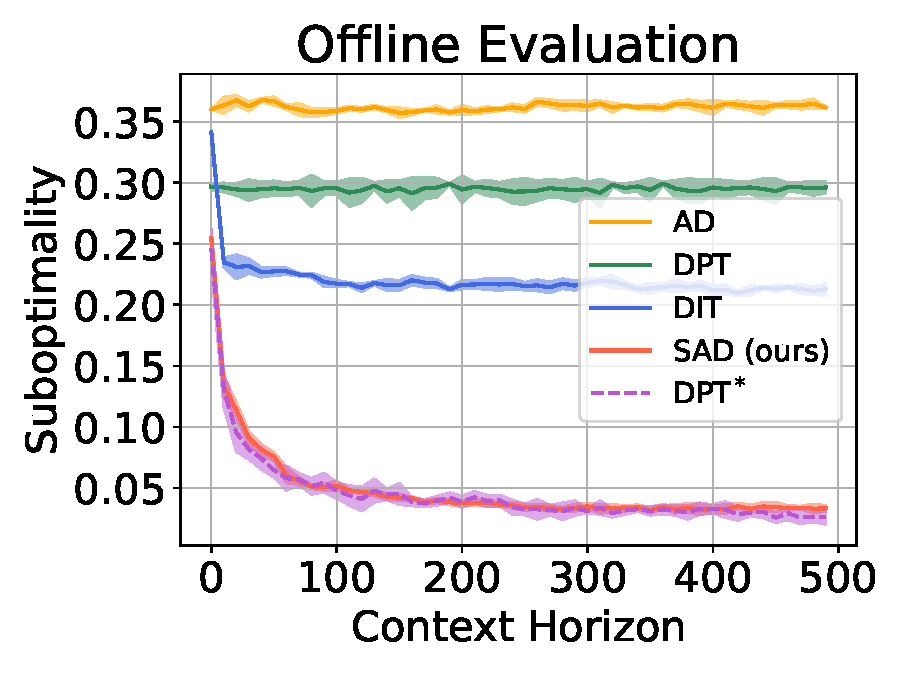
\includegraphics[width=0.25\columnwidth]{figures/plot_offline_bandits_gaussian.pdf}
% \!\!\!\!
% 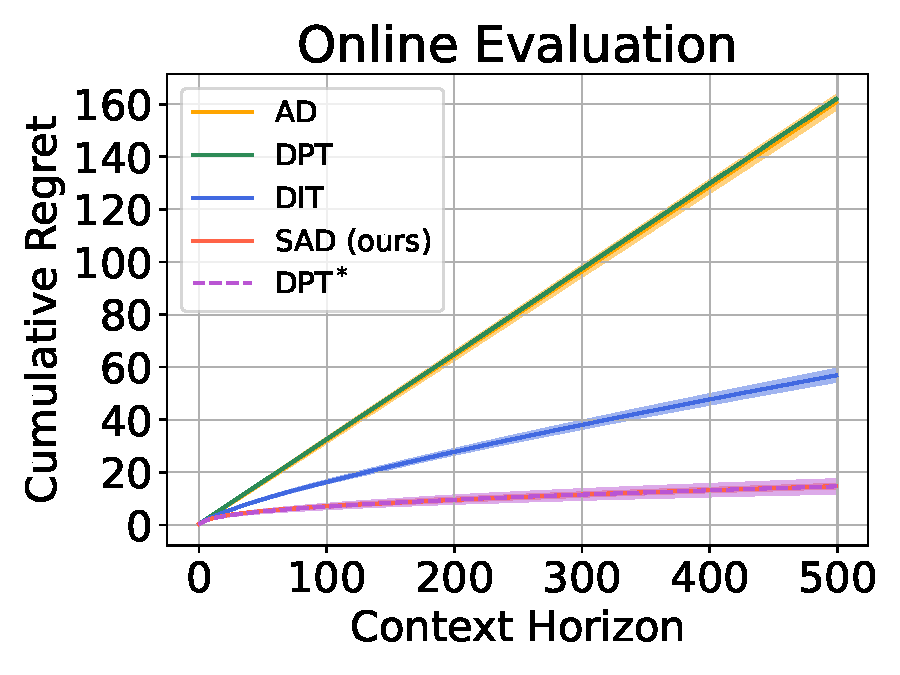
\includegraphics[width=0.25\columnwidth]{figures/plot_online_bandits_gaussian.pdf}
% \!\!\!\!
% 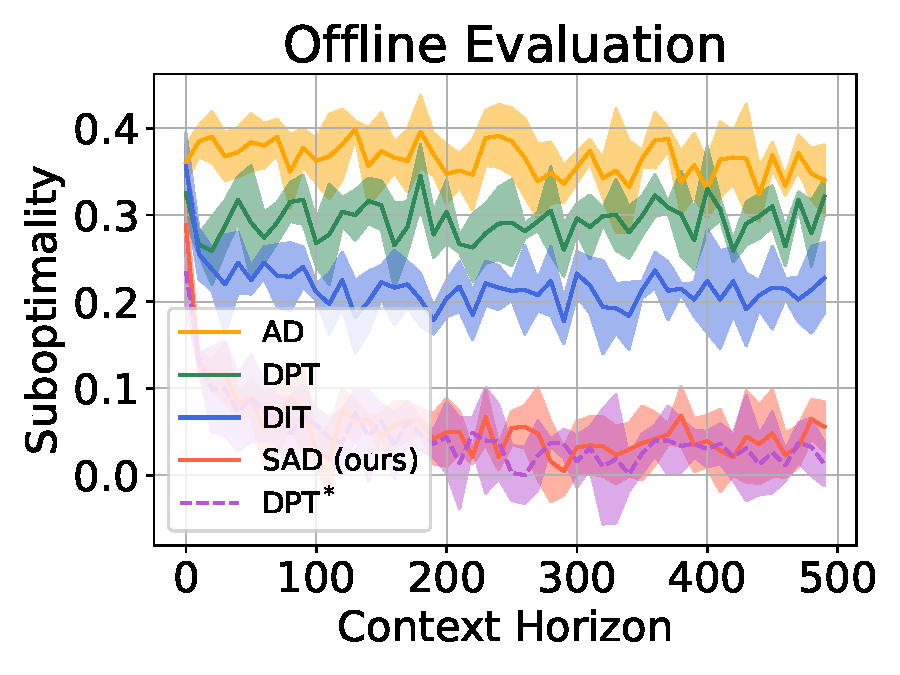
\includegraphics[width=0.25\columnwidth]{figures/plot_offline_bandits_bernoulli.pdf}
% \!\!\!\!
% 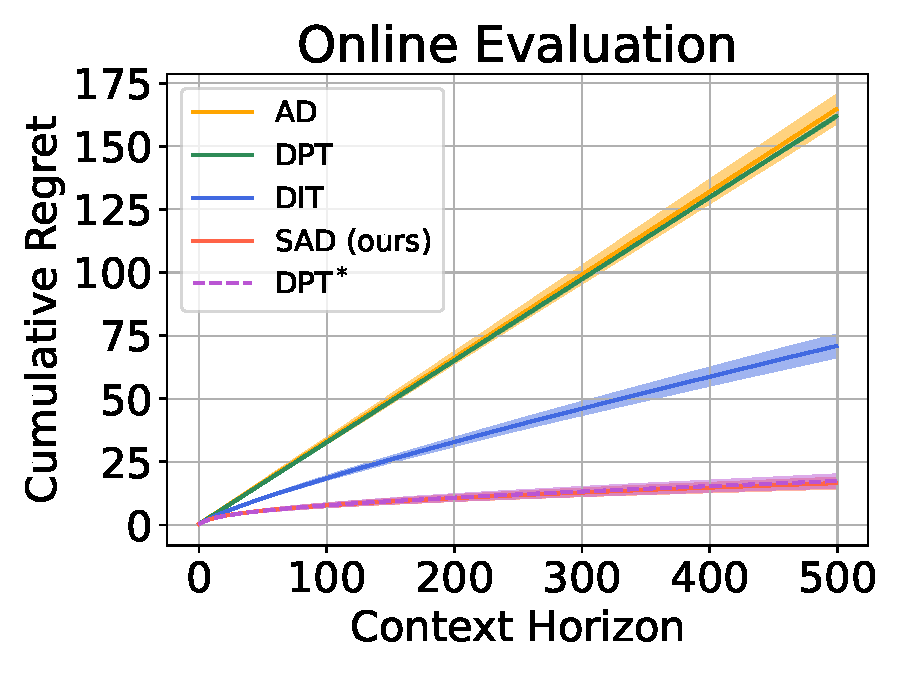
\includegraphics[width=0.25\columnwidth]{figures/plot_online_bandits_bernoulli.pdf}
% % \Description{bandits}
% \caption{Offline and online evaluations of ICRL algorithms trained under a uniform random policy: AD, DPT, DIT, DPT$^*$, and SAD (ours). Each algorithm contains four independent runs with mean and standard deviation. Environment: \textit{Gaussian Bandits} (left two), \textit{Bernoulli Bandits} (right two).}
% \label{fig_bandits}
% \end{figure}

%%%%%%%%%%%%%%%%
\begin{figure}[ht]
\centering 
\setcounter{subfigure}{0}
\subfigure[]
{
	\begin{minipage}{0.25\linewidth}
	\centering 
	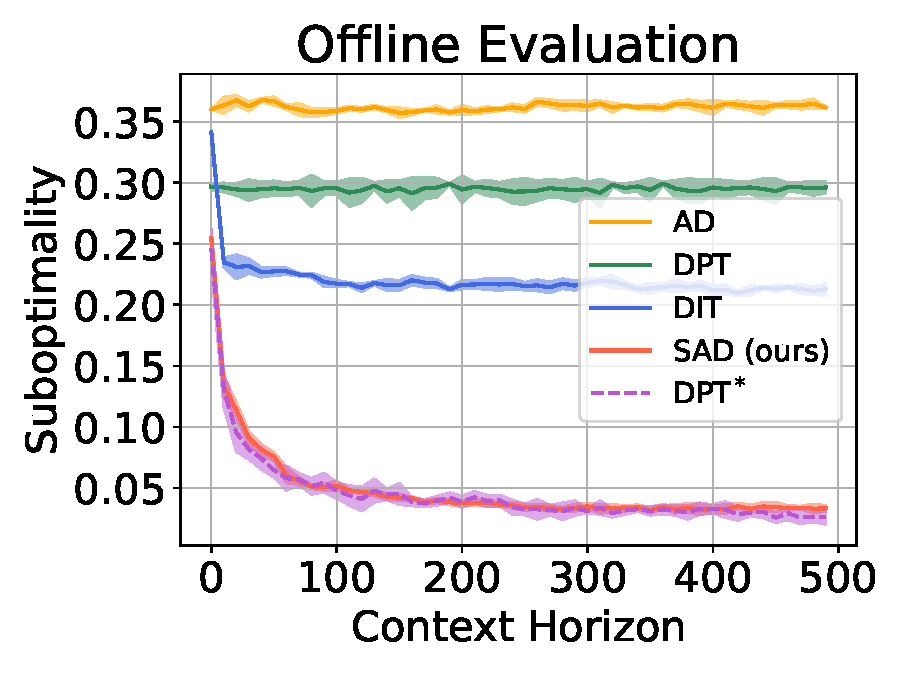
\includegraphics[width=\columnwidth]{figures/plot_offline_bandits_gaussian.pdf}
	\end{minipage}
}
\!\!\!\!\!\!\!\!\!
\subfigure[]
{
	\begin{minipage}{0.25\linewidth}
	\centering 
	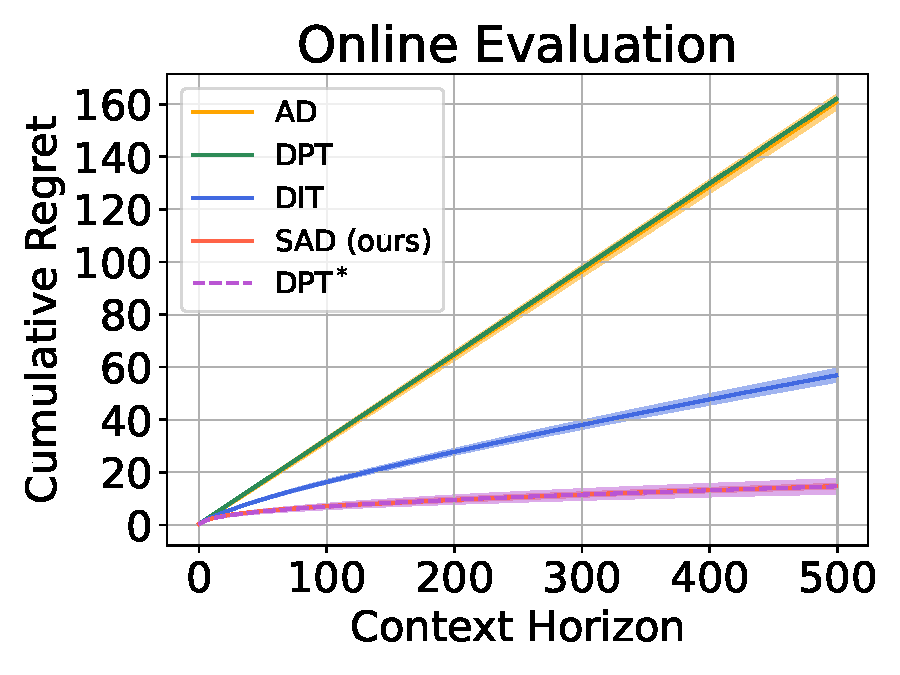
\includegraphics[width=\columnwidth]{figures/plot_online_bandits_gaussian.pdf}
	\end{minipage}
}
\!\!\!\!\!\!\!\!\!
\subfigure[]
{
	\begin{minipage}{0.25\linewidth}
	\centering 
	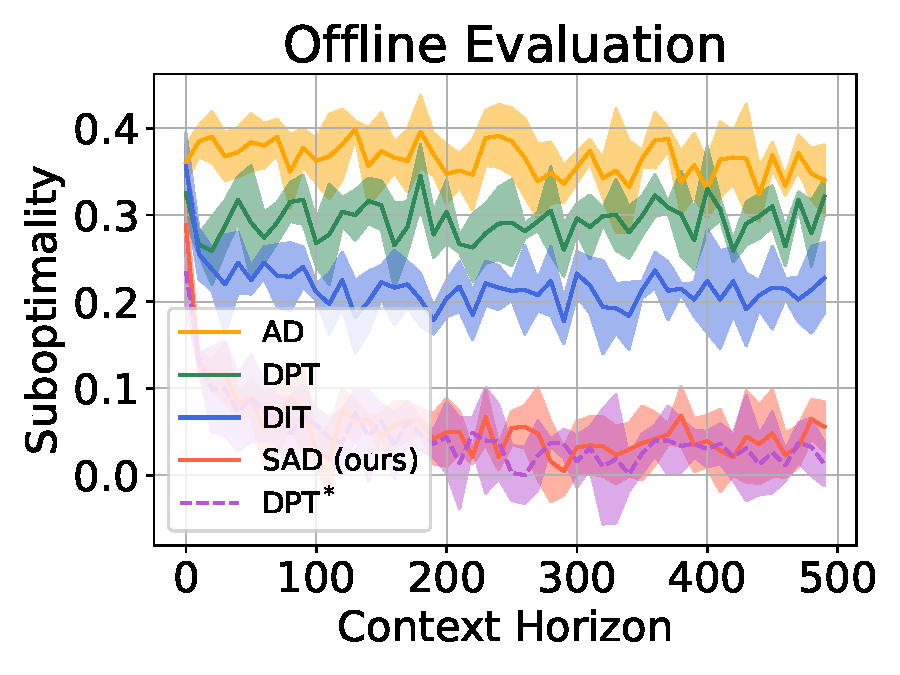
\includegraphics[width=\columnwidth]{figures/plot_offline_bandits_bernoulli.pdf}
	\end{minipage}
}
\!\!\!\!\!\!\!\!\!
\subfigure[]
{
	\begin{minipage}{0.25\linewidth}
	\centering 
	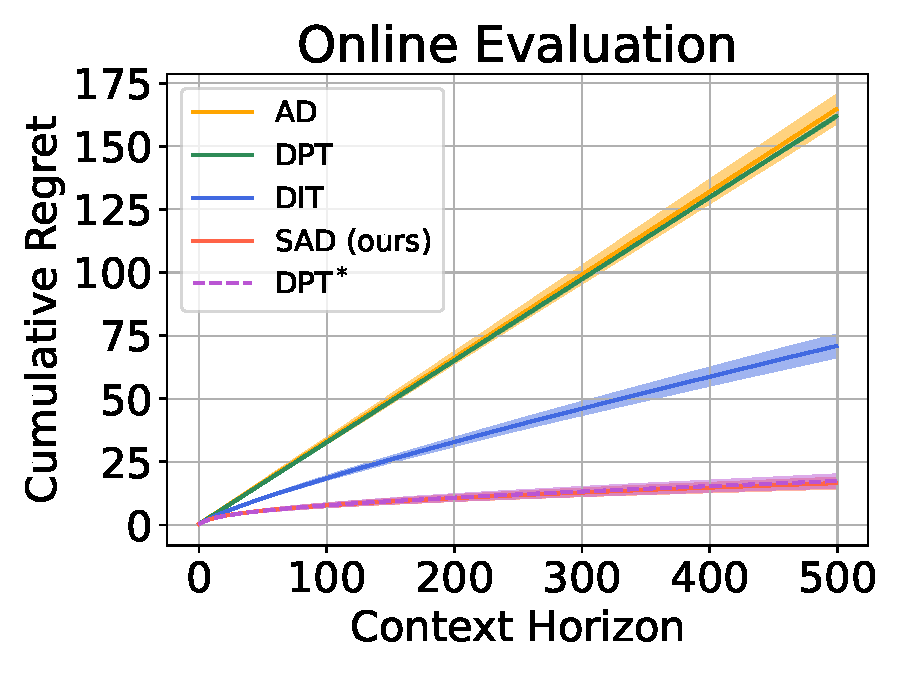
\includegraphics[width=\columnwidth]{figures/plot_online_bandits_bernoulli.pdf}
	\end{minipage}
}
\caption{Offline and online evaluations of ICRL algorithms trained under a uniform random policy: AD, DPT, DIT, DPT$^*$, and SAD (ours). Each algorithm contains four independent runs with mean and standard deviation. \textit{Gaussian Bandits}: (a) and (b), \textit{Bernoulli Bandits}: (c) and (d).}
\label{fig_bandits}
\end{figure}
%%%%%%%%%%%%%%%%


\paragraph{\textit{Bandits}.}
%
We adhere to offline and online evaluation metrics for \textit{Bandits} established in~\citep{lee2024supervised}. In the offline evaluation, we utilize the \textit{suboptimality} over different context horizon, defined by $\mu_{a^*} - \mu_a$, where $\mu_{a^*}$ and $\mu_a$ represent the mean rewards over 200 test environments of the optimal arm and the selected arm, respectively. In online evaluation, we employ \textit{cumulative regret}, defined by $\sum_{t=0}^T (\mu_{a^*} - \mu_{a_t})$,
%
% \blue{From the plot it looks like the sum is divided by $T$ at least in the offline evaluation.} \purple{In the offline evaluation, we compute the difference between the optimal policy and our policy given different horizon (Data in the x-axis, it is probably better to change the name of x-axis) So the x is not the episodes. It is the context horizon length. No matter x=0 or x=500, they are all run for 200 episodes, and take the mean.}
%
where $a_t$ denotes the selected arm at time $t$.
%
Figures~\ref{fig_bandits}(a) and \ref{fig_bandits}(b) demonstrate that our SAD approach significantly outperforms three SOTA baselines under uniform random policy, by achieving much lower \textit{suboptimality} and \textit{cumulative regret}.
%
More specifically, let us define the performance improvement of SAD over baselines in the offline evaluation by 
$(suboptimality_\text{baseline} - suboptimality_\text{SAD}) / suboptimality_\text{SAD}$.
%
% \begin{align}\label{eqn_perform_improve_bandit}
%     \frac{suboptimality_\text{baseline} - suboptimality_\text{SAD}}{suboptimality_\text{SAD}}.
% \end{align}
Likewise, the performance improvement in the online evaluation is to simply replace the \textit{suboptimality} by \textit{cumulative regret}. Then, SAD surpasses the best baseline, DIT, by achieving $354.0\%$ performance improvements in the offline evaluation and $273.9\%$ in the online evaluation (refer to the first row of Tables~\ref{tab_compare_offline} and \ref{tab_compare_online} in Appendix~\ref{appendix_experiment_detail_addition_result}).
%
To evaluate the out-of-distribution performance of SAD compared to other baselines, we test the models pretrained by all methods on the \textit{Gaussian Bandits} and assess their performance on the \textit{Bernoulli Bandits} with no further fine-tuning. Figures~\ref{fig_bandits}(c) and \ref{fig_bandits}(d) illustrate that SAD still achieves lower \textit{suboptimality} and \textit{cumulative regret} than all other baselines, demonstrating a more robust performance in handling out-of-distribution scenarios.
%
More specifically, SAD surpasses the best baseline, DIT, by $289.5\%$ in the offline evaluation and $313.9\%$ in the online evaluation (refer to the second row of Tables~\ref{tab_compare_offline} and \ref{tab_compare_online} in Appendix~\ref{appendix_experiment_detail_addition_result}).


In the environments of \textit{Darkroom} and \textit{Miniworld}, we use return as the evaluation metric. Moreover, we define the performance improvement of our SAD approach over the baseline methods in both offline and online evaluations by 
$(Return_\text{SAD} - Return_\text{baseline}) / Return_\text{baseline}$.
%
% \begin{align}\label{eqn_perform_improve_mdp}
%     \frac{Return_\text{SAD} - Return_\text{baseline}}{Return_\text{baseline}}.
% \end{align}


% \begin{figure}[ht]
% \centering 
% \includegraphics[width=0.25\columnwidth]{figures/plot_offline_darkroom7_7.pdf}  
% \!\!\!\!
% \includegraphics[width=0.25\columnwidth]{figures/plot_online_darkroom7_7.pdf}
% \!\!\!\!
% \includegraphics[width=0.25\columnwidth]{figures/plot_offline_darkroom10_10.pdf} 
% \!\!\!\!
% \includegraphics[width=0.25\columnwidth]{figures/plot_online_darkroom10_10.pdf}  
% % \Description{DarkRoom}
% \caption{Offline and online evaluations of ICRL algorithms trained under a uniform random policy: AD, DPT, DIT, DPT$^*$, and SAD (ours). Each algorithm contains four independent runs with mean and standard deviation. Environment: \textit{DarkRoom} (left two), \textit{DarkRoom-Large} (right two).}
% \label{fig_darkroom}
% \end{figure}


%%%%%%%%%%%%%%%%
\begin{figure}[ht]
\centering 
\setcounter{subfigure}{0}
\subfigure[]
{
	\begin{minipage}{0.25\linewidth}
	\centering 
	\includegraphics[width=\columnwidth]{figures/plot_offline_darkroom7_7.pdf}
	\end{minipage}
}
\!\!\!\!\!\!\!\!\!
\subfigure[]
{
	\begin{minipage}{0.25\linewidth}
	\centering 
	\includegraphics[width=\columnwidth]{figures/plot_online_darkroom7_7.pdf}
	\end{minipage}
}
\!\!\!\!\!\!\!\!\!
\subfigure[]
{
	\begin{minipage}{0.25\linewidth}
	\centering 
	\includegraphics[width=\columnwidth]{figures/plot_offline_darkroom10_10.pdf}
	\end{minipage}
}
\!\!\!\!\!\!\!\!\!
\subfigure[]
{
	\begin{minipage}{0.25\linewidth}
	\centering 
	\includegraphics[width=\columnwidth]{figures/plot_online_darkroom10_10.pdf}
	\end{minipage}
}
\caption{Offline and online evaluations of ICRL algorithms trained under a uniform random policy: AD, DPT, DIT, DPT$^*$, and SAD (ours). Each algorithm contains four independent runs with mean and standard deviation. \textit{DarkRoom}: (a) and (b). \textit{DarkRoom-Large}: (c) and (d).}
\label{fig_darkroom}
\end{figure}
%%%%%%%%%%%%%%%%



\paragraph{\textit{Darkrooms}.}

% We use return as the evaluation metric for both \textit{Darkroom} and \textit{Darkroom-Large}.
%
Figure~\ref{fig_darkroom} demonstrates that our SAD approach significantly outperforms three SOTA baselines in the \textit{Darkroom} and \textit{Darkroom-Large} under uniform random policy, by achieving much higher return. 
%
In the \textit{Darkroom}, SAD surpasses the best baseline, DIT, by $149.3\%$ in the offline evaluation and $41.7\%$ in the online evaluation (refer to the third row of Tables~\ref{tab_compare_offline} and \ref{tab_compare_online} in Appendix~\ref{appendix_experiment_detail_addition_result}).
%
Likewise, in the \textit{Darkroom-Large}, SAD outperforms the best baseline, DIT, by $266.8\%$ in the offline evaluation and $24.7\%$ in the online evaluation (refer to the fourth row of Tables~\ref{tab_compare_offline} and \ref{tab_compare_online} in Appendix~\ref{appendix_experiment_detail_addition_result}).




% \begin{figure}[ht]
% \centering 
% 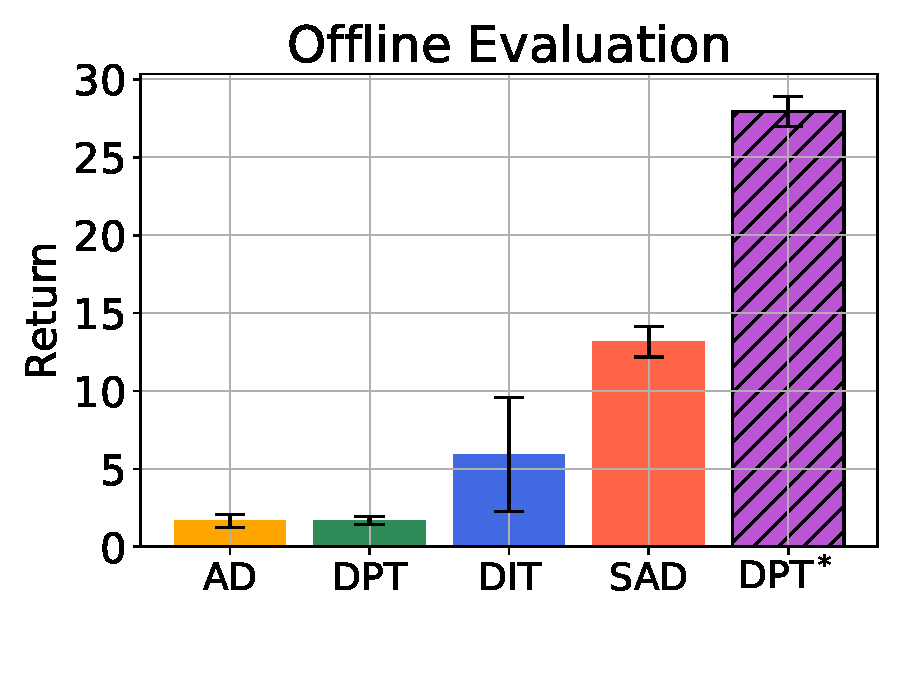
\includegraphics[width=0.25\columnwidth]{figures/plot_offline_miniworld.pdf}  
% % \!\!\!
% 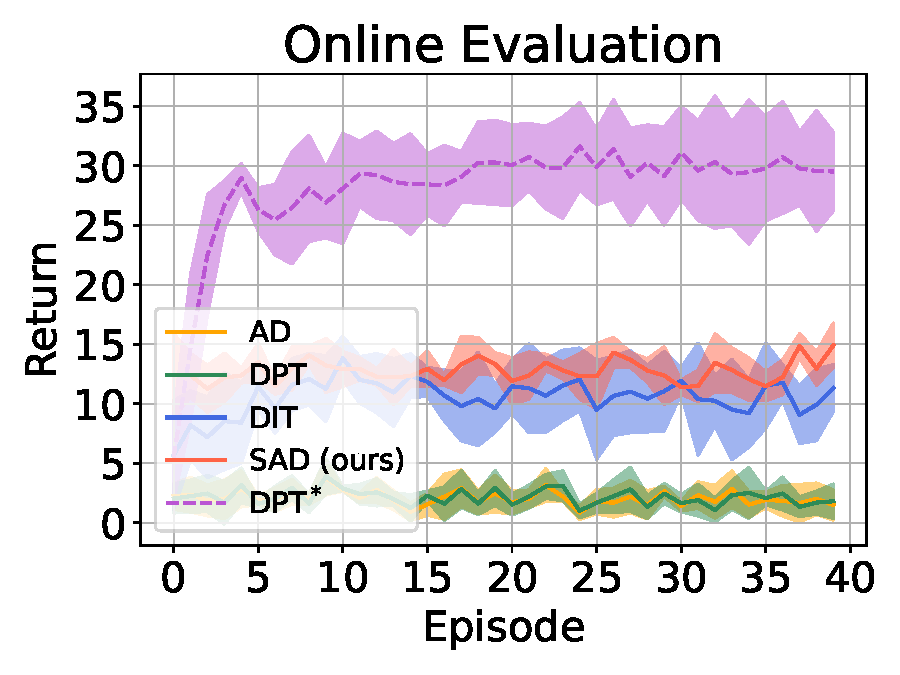
\includegraphics[width=0.25\columnwidth]{figures/plot_online_miniworld.pdf}  
% % \Description{\textit{Miniworld}}
% \caption{Offline and online evaluations of ICRL algorithms trained under a uniform random policy: AD, DPT, DIT, DPT$^*$, and SAD (ours). Each algorithm contains four independent runs with mean and standard deviation. Environment: \textit{Miniworld}.}
% \label{fig_miniworld}
% \end{figure}


%%%%%%%%%%%%%%%%
\begin{figure}[ht]
\centering 
\setcounter{subfigure}{0}
\subfigure[]
{
	\begin{minipage}{0.25\linewidth}
	\centering 
	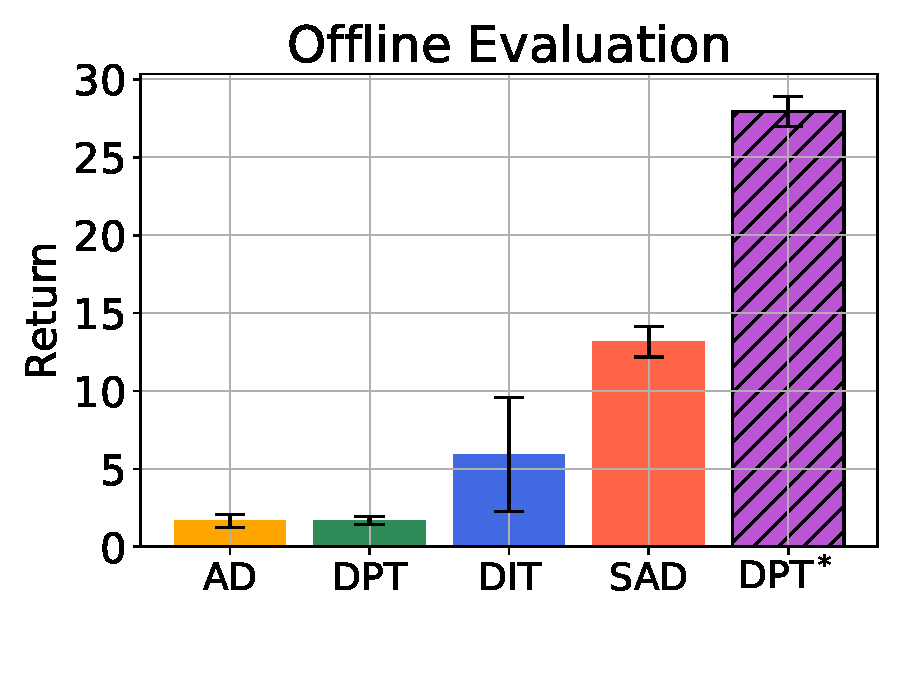
\includegraphics[width=\columnwidth]{figures/plot_offline_miniworld.pdf}
	\end{minipage}
}
% \!\!\!\!\!\!\!\!\!
\subfigure[]
{
	\begin{minipage}{0.25\linewidth}
	\centering 
	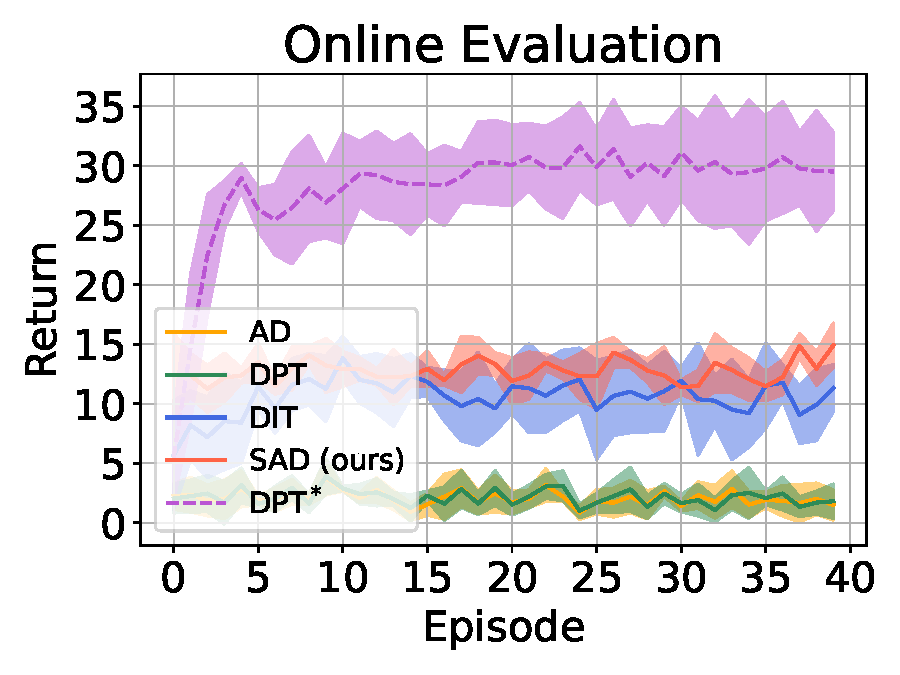
\includegraphics[width=\columnwidth]{figures/plot_online_miniworld.pdf}
	\end{minipage}
}
\caption{Offline and online evaluations of ICRL algorithms trained under a uniform random policy: AD, DPT, DIT, DPT$^*$, and SAD (ours). Each algorithm contains four independent runs with mean and standard deviation. Environment: \textit{Miniworld}.}
\label{fig_miniworld}
\end{figure}
%%%%%%%%%%%%%%%%



\paragraph{\textit{Miniworld}.}

% Similar to the \textit{Darkroom} environment, we consider return as the evaluation metric for \textit{Miniworld}.
%
Figure~\ref{fig_miniworld} demonstrates that our SAD approach outperforms the three SOTA baselines in the \textit{Miniworld} under uniform random policy, by achieving a higher return. 
%
More specifically, SAD surpasses the best baseline, DIT, by $122.1\%$ in the offline evaluation and $21.7\%$ in the online evaluation (refer to the fifth row of Tables~\ref{tab_compare_offline} and \ref{tab_compare_online} in Appendix~\ref{appendix_experiment_detail_addition_result}).



Tables~\ref{tab_compare_offline} and \ref{tab_compare_online} also imply that SAD significantly outperforms all baselines on average across the five ICRL benchmark environments. In the offline evaluation, SAD exceeds the best baseline DIT by $236.3\%$ on average, the second-best DPT by $2015.9\%$, and the third-best AD by $2075.2\%$. In the online evaluation, SAD surpasses DIT by $135.2\%$, DPT by $3093.8\%$, and AD by $3208.8\%$ on average.
%
%
In addition to comparing SAD with the three SOTA ICRL algorithms under the uniform random policy, we also include the empirical performance of the DPT with optimal action labels (DPT$^*$) as the oracle upper bound of SAD. We observe that SAD demonstrates performance comparable to DPT$^*$ in tasks such as \textit{Gaussian Bandits}, \textit{Bernoulli Bandits}, \textit{DarkRoom}, and \textit{DarkRoom-Large}. Although \textit{Miniworld} introduces challenges due to its pixel-based inputs and complex environments, SAD under the random policy still achieves approximately $50\%$ of the performance of DPT$^*$. Overall, SAD is within $18.6\%$ of the performance of DPT$^*$ in the offline evaluation across five ICRL tasks, and within $12.3\%$ in the online evaluation (see details in Tables~\ref{tab_compare_offline} and \ref{tab_compare_online}).









\subsection{Ablation Studies}
\label{subsec_ablation}


\paragraph{Trust Horizon.}
%
%
Theorems~\ref{theorem_mab} implies that the uniform random policy is probabilistically trustworthy within a horizon $N$, with monotonically increasing probability of selecting the optimal action with $N$ in the MAB problem. We substantiate this observation from the theorem by empirical evidence, as presented in Figure~\ref{fig_action_select_acc}(a).
%
Furthermore, we conduct empirical investigations into the influence of the trust horizon $N$ on the performance of the MAB problem, which considers the environments of \textit{Gaussian Bandits}.
%
As expected, a larger $N$ in the MAB problem leads to a better performance (see Figures~\ref{fig_diff_trust_horizon}(a) and \ref{fig_diff_trust_horizon}(b)).


% \begin{figure}[ht]
% \centering 
% 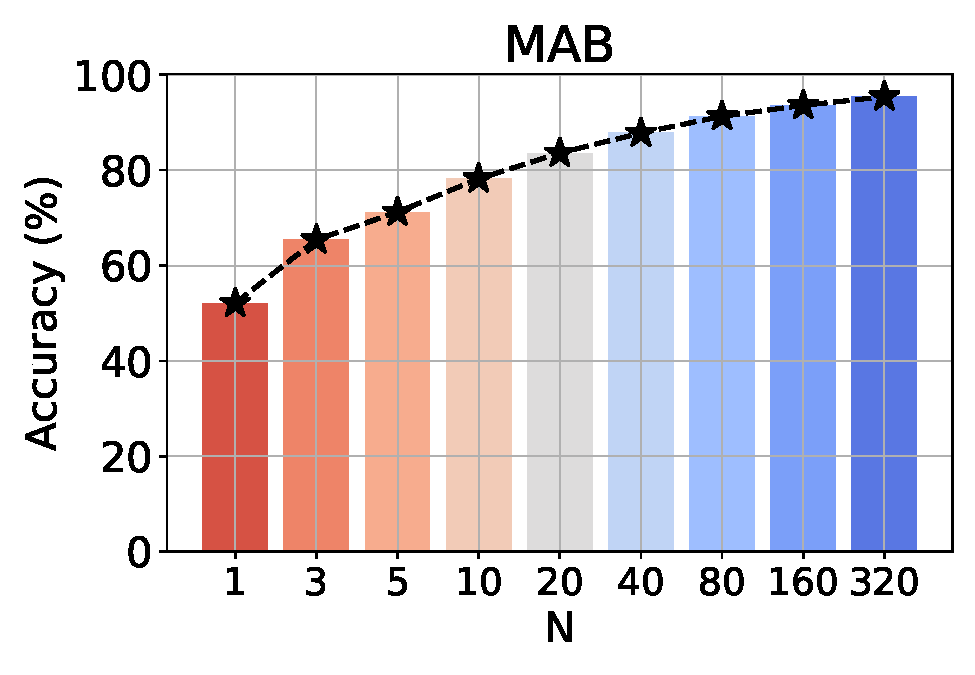
\includegraphics[width=0.25\columnwidth]{figures/plot_action_select_acc_MAB.pdf}
% %\!\!
% 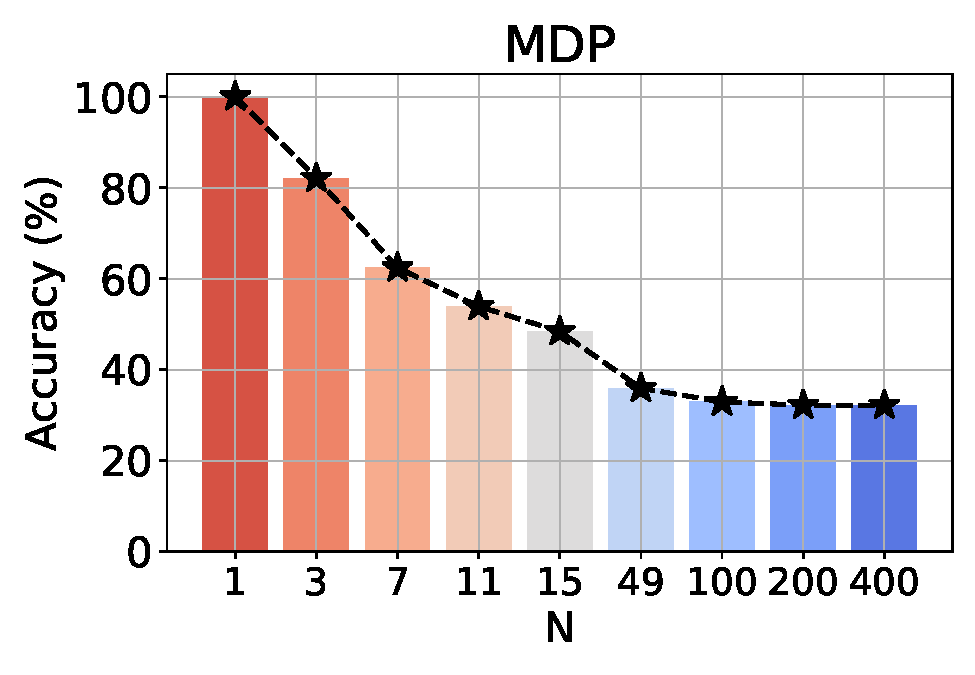
\includegraphics[width=0.25\columnwidth]{figures/plot_action_select_acc_MDP.pdf}
% \caption{The accuracy (probability) of selecting the optimal action in the MAB and MDP with varying trust horizon $N$.}
% \label{fig_action_select_acc}
% \end{figure}


%%%%%%%%%%%%%%%%
\begin{figure}[ht]
\centering 
\setcounter{subfigure}{0}
\!\!
\subfigure[]
{
	\begin{minipage}{0.25\linewidth}
	\centering 
	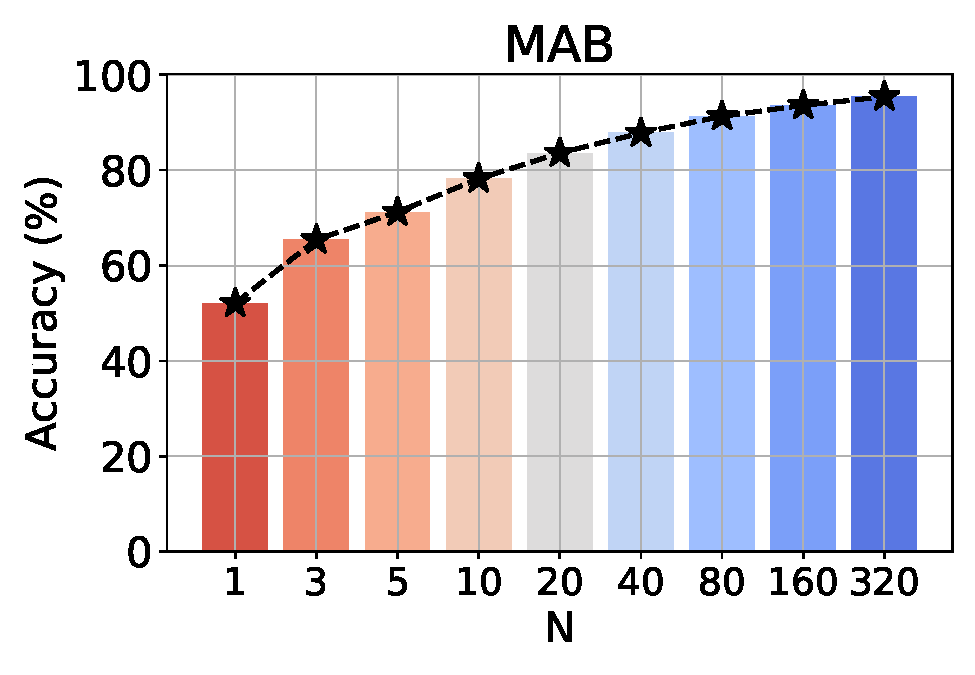
\includegraphics[width=\columnwidth]{figures/plot_action_select_acc_MAB.pdf}
	\end{minipage}
}
\!\!
\subfigure[]
{
	\begin{minipage}{0.25\linewidth}
	\centering 
	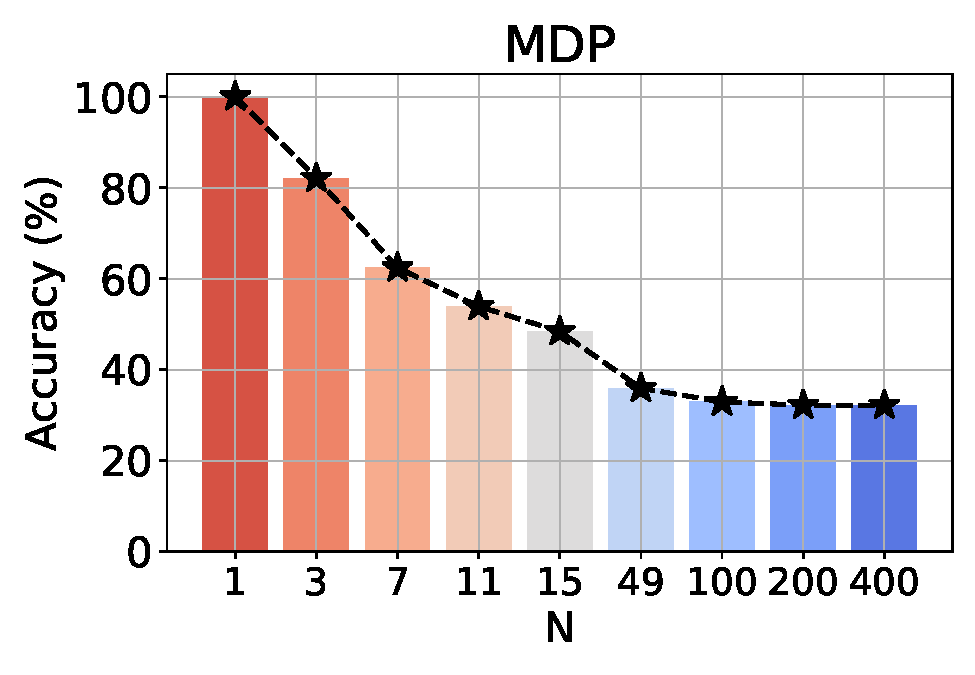
\includegraphics[width=\columnwidth]{figures/plot_action_select_acc_MDP.pdf}
	\end{minipage}
}
\!\!\!
\subfigure[]
{
	\begin{minipage}{0.22\linewidth}
	\centering 
	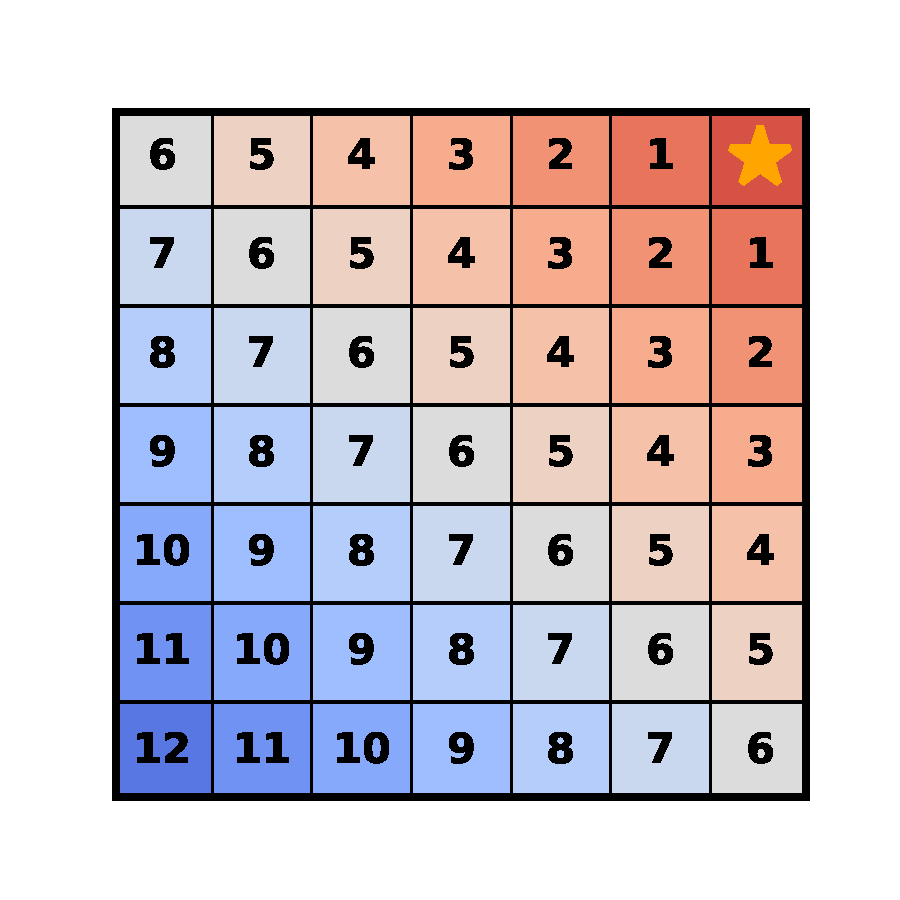
\includegraphics[width=0.855\columnwidth]{figures/grid_world_demo_corner.pdf}
	\end{minipage}
}
\!\!\!\!\!
\subfigure[]
{
	\begin{minipage}{0.22\linewidth}
	\centering 
	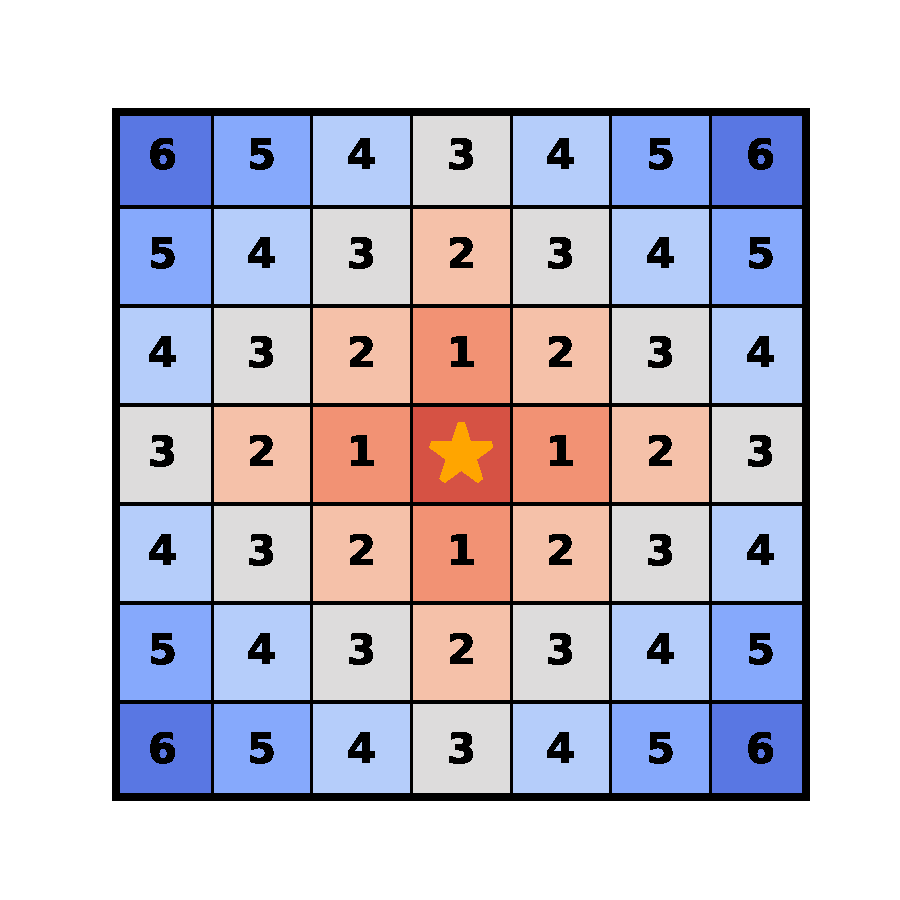
\includegraphics[width=0.855\columnwidth]{figures/grid_world_demo_middle.pdf}
	\end{minipage}
}
\caption{(a) and (b): The accuracy (probability) of selecting the optimal action in the MAB and MDP problems with varying trust horizon $N$. (c) and (d): The minimal number of steps required for a query state to reach the goal (the golden star) in the upper-right corner and in the middle.}
\label{fig_action_select_acc}
\end{figure}
%%%%%%%%%%%%%%%%










% \begin{figure}[ht]
% \centering 
% 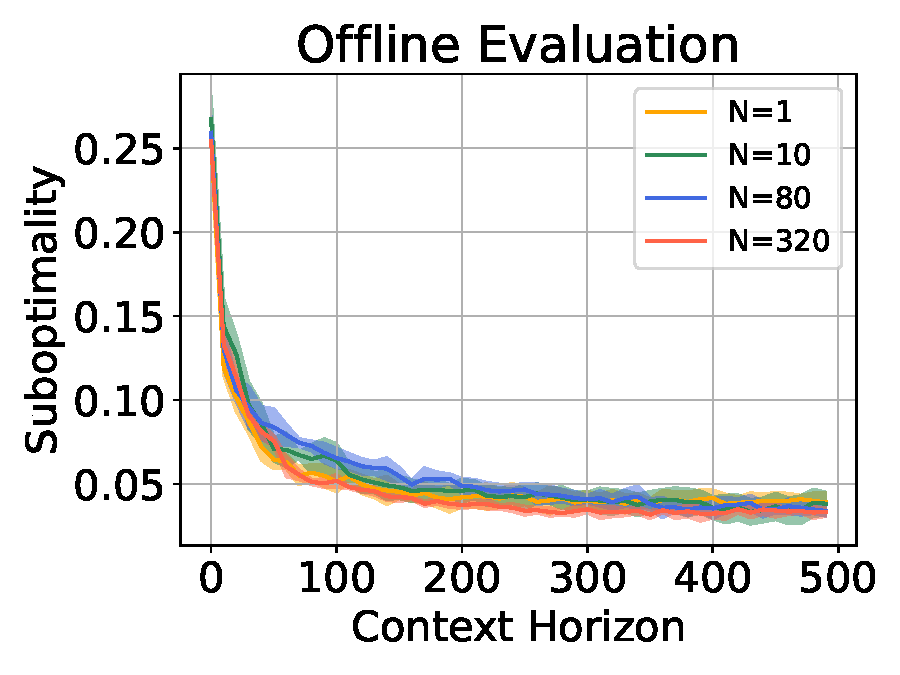
\includegraphics[width=0.25\columnwidth]{figures/plot_offline_bandits_different_N.pdf}
% \!\!\!\!
% 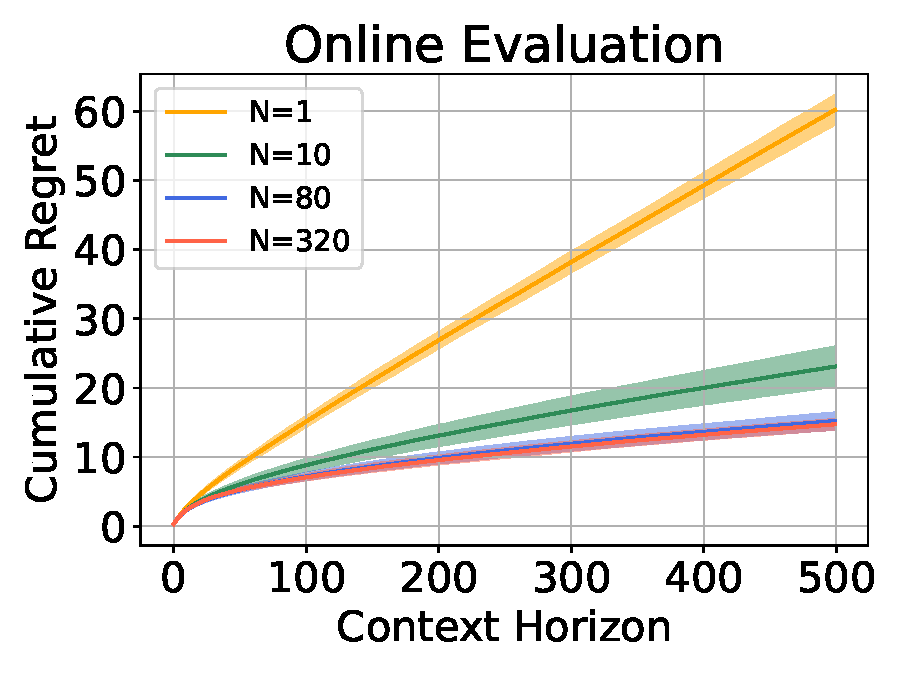
\includegraphics[width=0.25\columnwidth]{figures/plot_online_bandits_different_N.pdf}
% \!\!\!\!
% 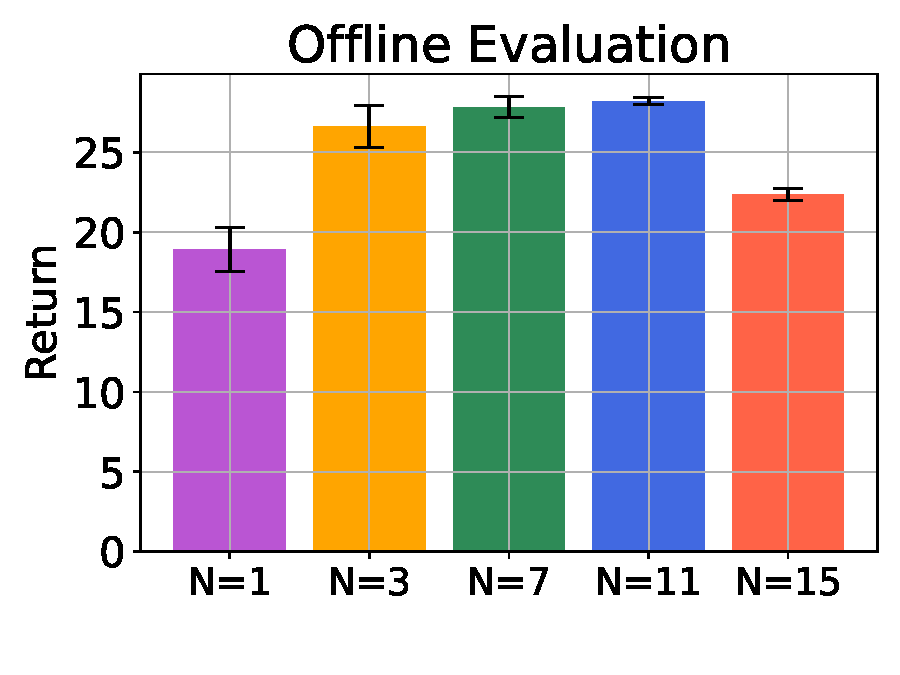
\includegraphics[width=0.25\columnwidth]{figures/plot_offline_different_N.pdf}
% \!\!\!\!
% 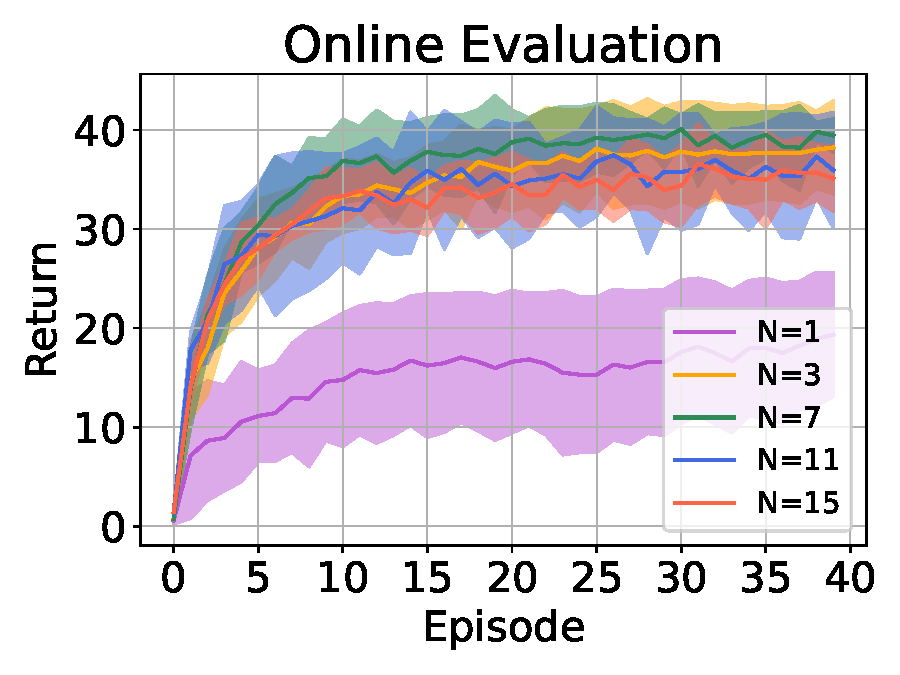
\includegraphics[width=0.25\columnwidth]{figures/plot_online_different_N.pdf}
% % \Description{DarkRoom}
% \caption{Offline and online evaluation of SAD with varying trust horizon $N$ for MAB (left two) and MDP (right two). Each $N$ contains four independent runs with mean and standard deviation.}
% \label{fig_diff_trust_horizon}
% \end{figure}



%%%%%%%%%%%%%%%%
\begin{figure}[ht]
\centering 
\setcounter{subfigure}{0}
\subfigure[]
{
	\begin{minipage}{0.25\linewidth}
	\centering 
	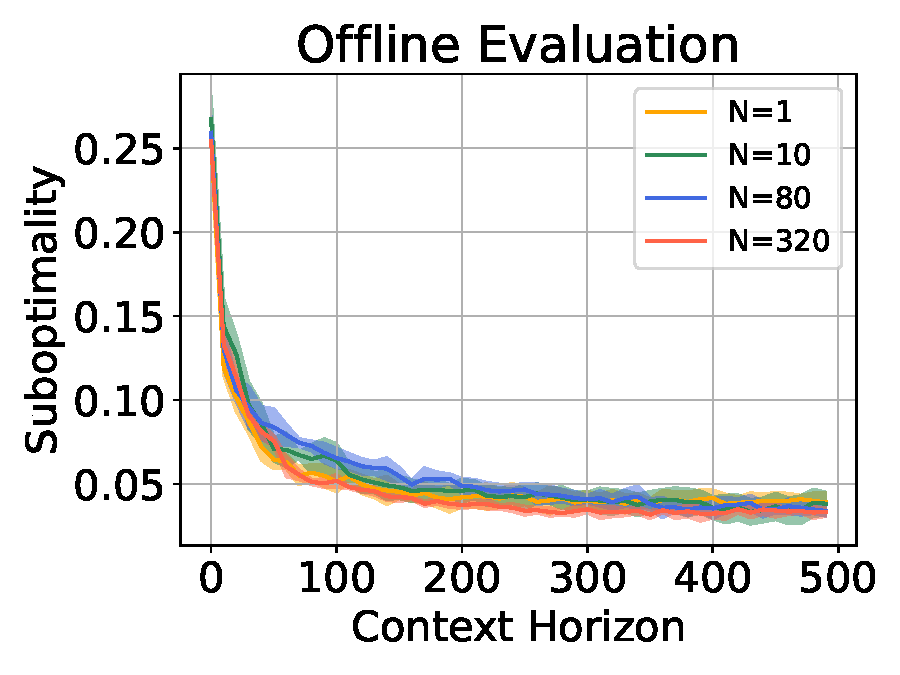
\includegraphics[width=\columnwidth]{figures/plot_offline_bandits_different_N.pdf}
	\end{minipage}
}
\!\!\!\!\!\!\!\!\!
\subfigure[]
{
	\begin{minipage}{0.25\linewidth}
	\centering 
	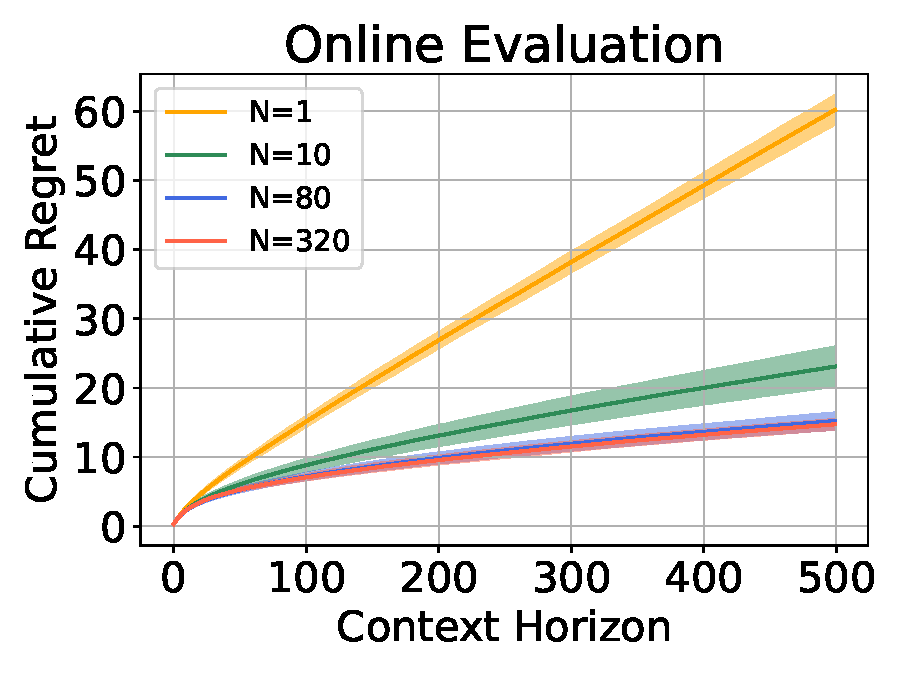
\includegraphics[width=\columnwidth]{figures/plot_online_bandits_different_N.pdf}
	\end{minipage}
}
\!\!\!\!\!\!\!\!\!
\subfigure[]
{
	\begin{minipage}{0.25\linewidth}
	\centering 
	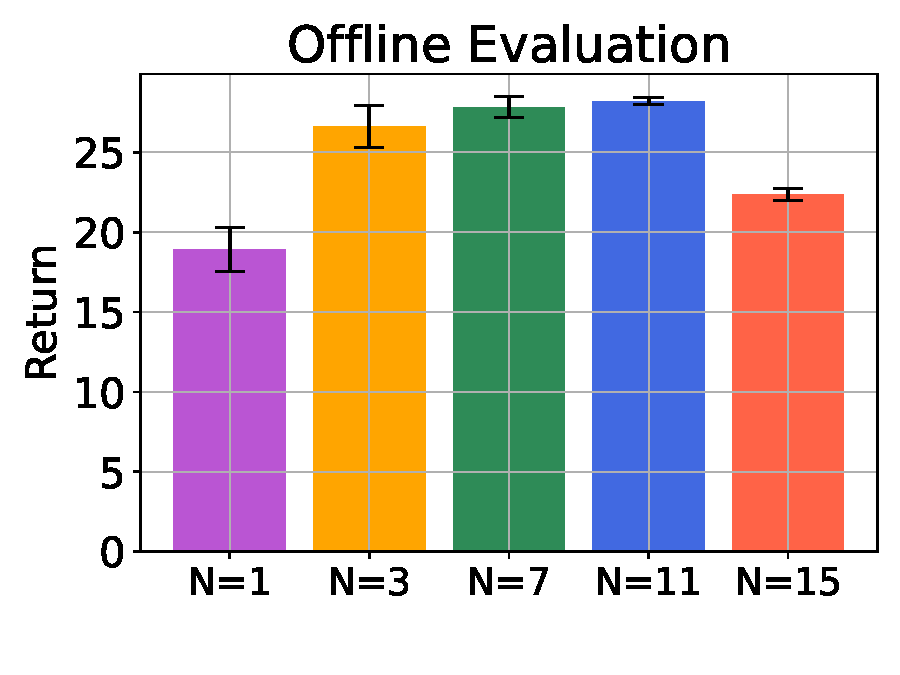
\includegraphics[width=\columnwidth]{figures/plot_offline_different_N.pdf}
	\end{minipage}
}
\!\!\!\!\!\!\!\!\!
\subfigure[]
{
	\begin{minipage}{0.25\linewidth}
	\centering 
	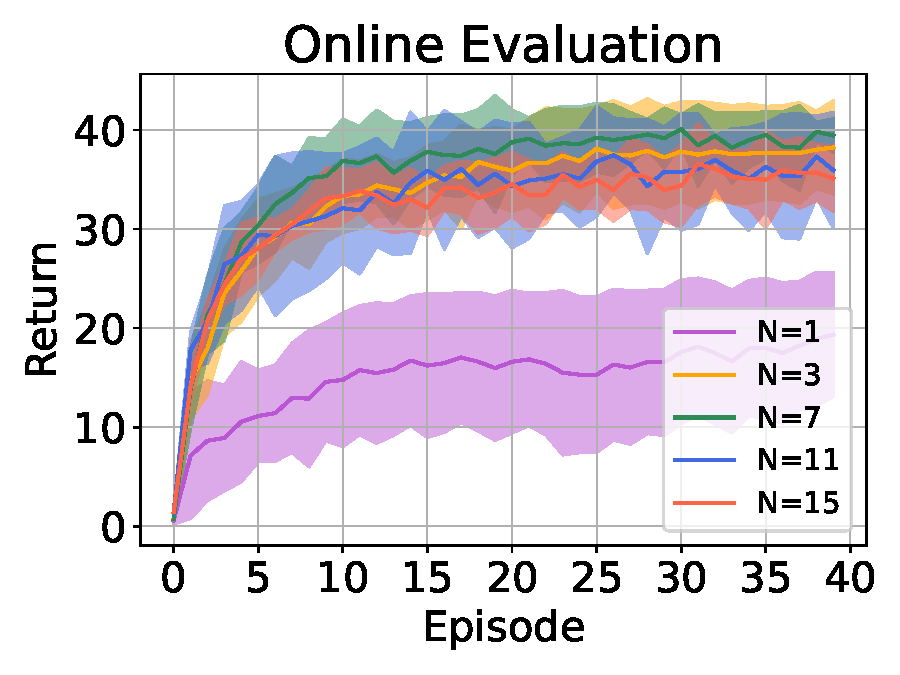
\includegraphics[width=\columnwidth]{figures/plot_online_different_N.pdf}
	\end{minipage}
}
\caption{Offline and online evaluation of SAD with varying trust horizon $N$ for MAB: (a) and (b), and for MDP: (c) and (d). Each $N$ contains four independent runs with mean and standard deviation.}
\label{fig_diff_trust_horizon}
\end{figure}
%%%%%%%%%%%%%%%%


We then shift to the MDP problem with the environment of \textit{Darkroom}.
Notice that in our practical algorithm for the sparse-reward MDP like \textit{Darkroom} (Algorithm~\ref{alg_collect_queries_sparse}), we only utilize the state-action pairs that can reach the goal within a trust horizon. Therefore, we solely record the probability/accuracy of selecting the optimal actions on those states, as presented in Figure~\ref{fig_action_select_acc}(b). It shows that the accuracy monotonically decreases with respect to the trust horizon $N$, which, at first glance, may lead to monotonically decreasing performance as well. Nonetheless, we acknowledge that this is not the case.
%
In particular, a large trust horizon $N$ in the MDP leads to the low accuracy of selecting the optimal action, whereas a small $N$ may induce the partially short-sighted training of FM, as Algorithm~\ref{alg_collect_queries_sparse} solely trains on the states at most $N$ steps from the goal, instead of all states (refer to Figures~\ref{fig_action_select_acc}(c) and \ref{fig_action_select_acc}(d)).
%
Our numerical results in Figures~\ref{fig_diff_trust_horizon}(c) and \ref{fig_diff_trust_horizon}(d) validate this with the fact $N=7$ performing best, and provide the empirical evidence that either an excessively large or small trust horizon can lead to suboptimality.
% \blue{I'm less convinced about this last comment. Are saying for short $N$ we have more optimality (in some states) and for large $N$ we have more trustworthy decisions?}
% \purple{Maybe it is not clear by saying the trade-off between trustworthiness and optimality. Maybe we can simply say that  ``\textit{either an excessively large or small N can lead to suboptimal outcomes}''}

% Notably, a smaller $N$ implies greater trustworthiness for the selected action. In the extreme case when $T=N=0$, selecting actions by maximizing the Q-value of a uniform random policy is equivalent to select actions by maximizing the Q-value of the optimal policy.
%
% However, it is not advisable to choose $N$ as small as possible, as a short horizon leads to short-sighted decisions that may deviate far from optimal actions~\citep{sutton2018reinforcement}.
%
% Indeed, in the practical implementation of solving the \textit{Darkroom} task, a small $N$ causes the agent to focus on querying states near the goal, as it must reach the goal within a short horizon. This results in the agent prioritizing state-action pairs that facilitate short-sighted decisions.
%



% \begin{figure}[ht]
% \centering 
% 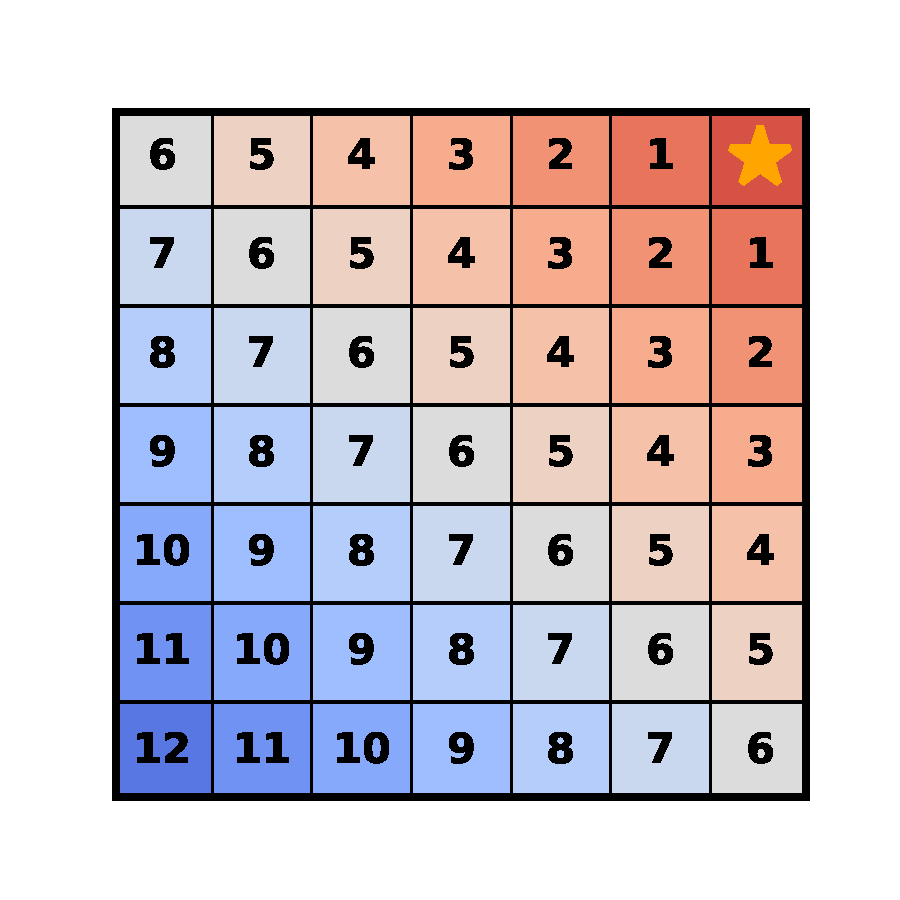
\includegraphics[width=0.25\columnwidth]{figures/grid_world_demo_corner.pdf}
% 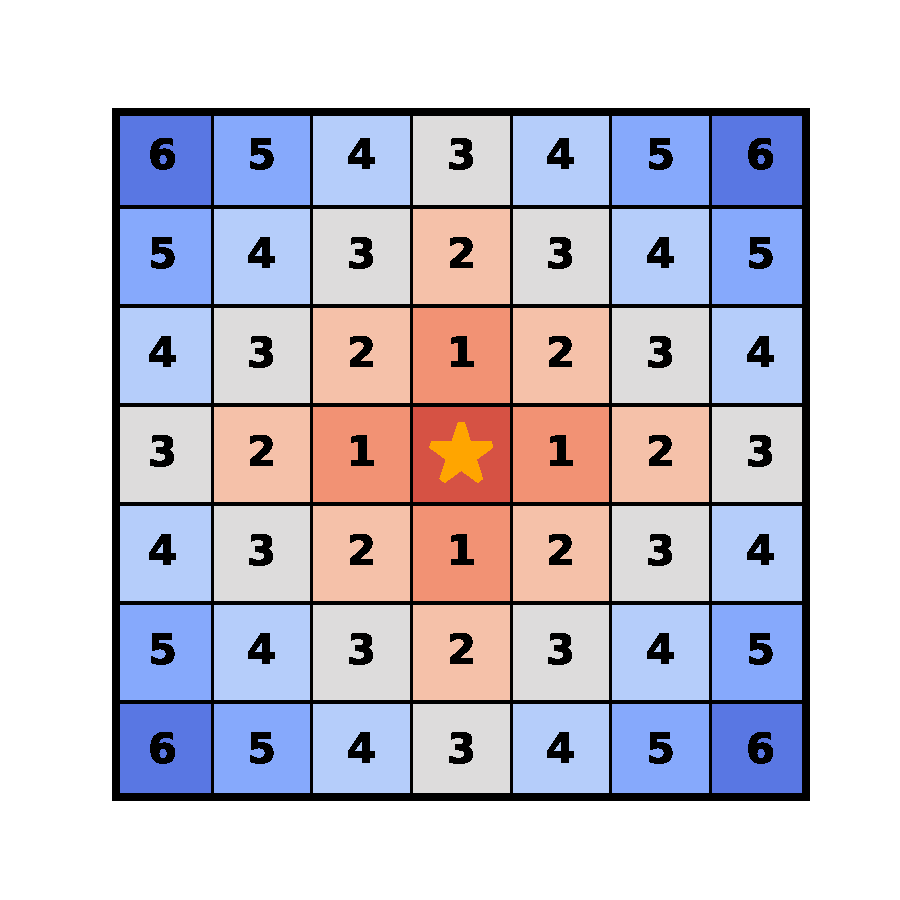
\includegraphics[width=0.25\columnwidth]{figures/grid_world_demo_middle.pdf}
% \caption{The minimal number of steps required for a query state to reach the goal (the golden star). Left: goal in the upper-right corner. Right: goal in the middle.}
% \label{fig_grid_world_demo}
% \end{figure}

% %%%%%%%%%%%%%%%%
% \begin{figure}[ht]
% \centering 
% \setcounter{subfigure}{0}
% \subfigure[]
% {
% 	\begin{minipage}{0.21\linewidth}
% 	\centering 
% 	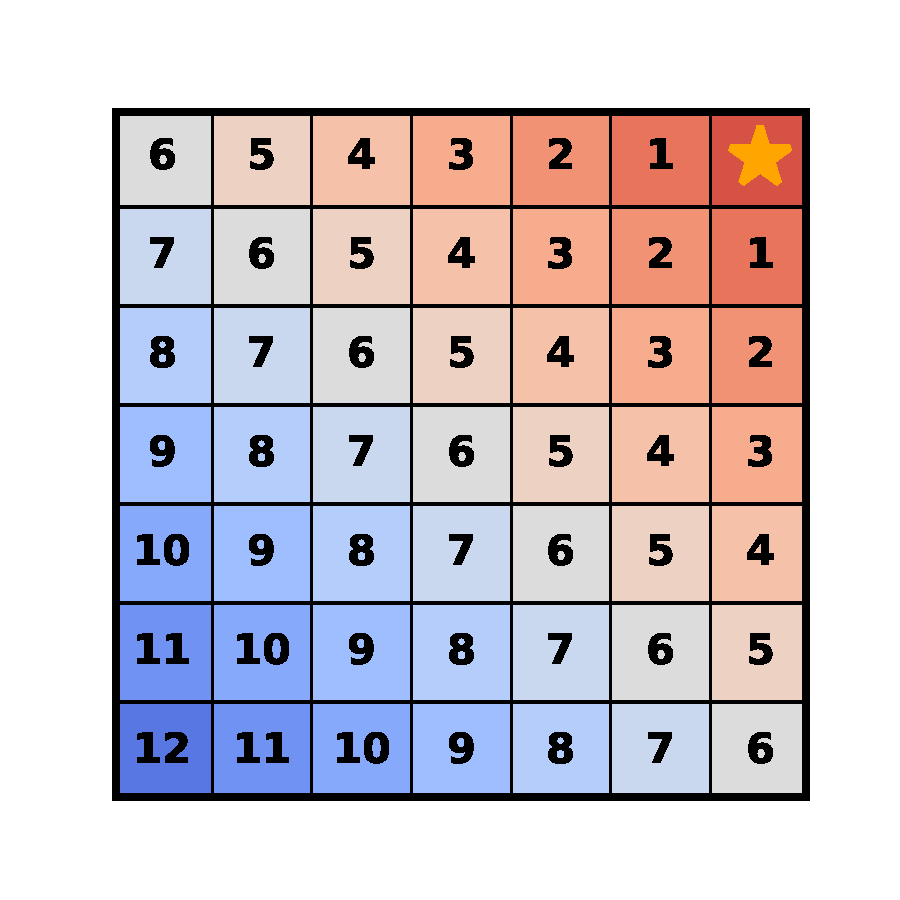
\includegraphics[width=\columnwidth]{figures/grid_world_demo_corner.pdf}
% 	\end{minipage}
% }
% % \!\!\!\!\!\!\!\!\!
% \subfigure[]
% {
% 	\begin{minipage}{0.21\linewidth}
% 	\centering 
% 	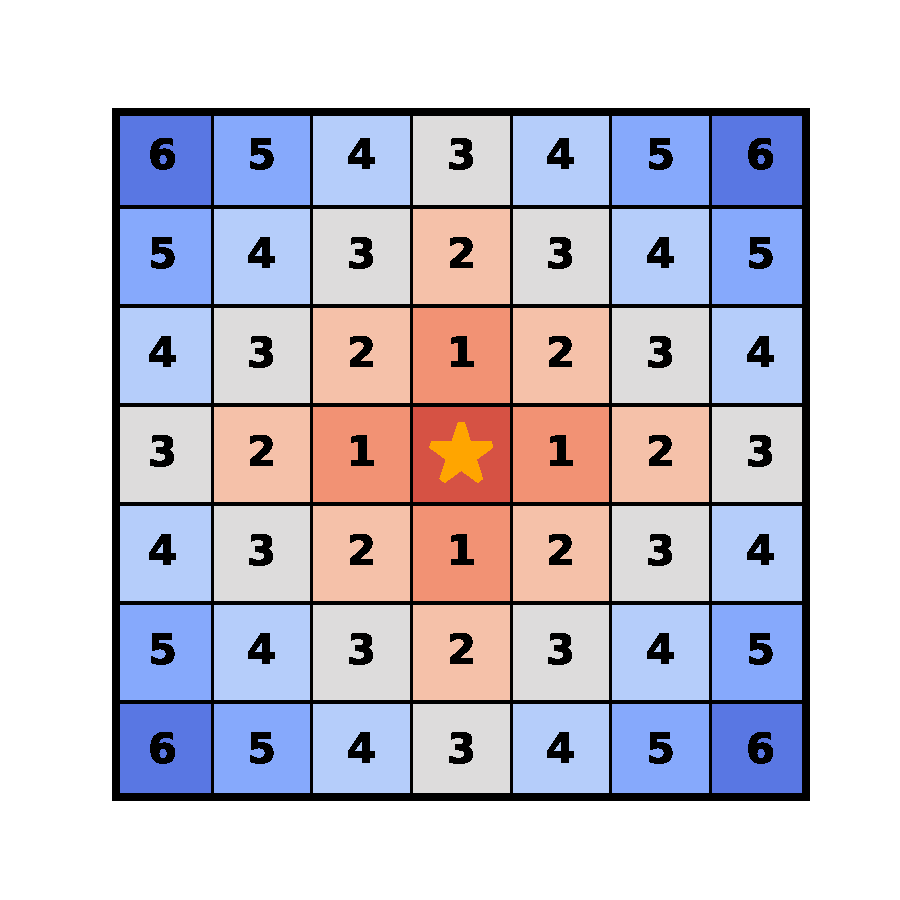
\includegraphics[width=\columnwidth]{figures/grid_world_demo_middle.pdf}
% 	\end{minipage}
% }
% \caption{The minimal number of steps required for a query state to reach the goal (the golden star). (a): goal in the upper-right corner. (b): goal in the middle.}
% \label{fig_grid_world_demo}
% \end{figure}
% %%%%%%%%%%%%%%%%


\paragraph{Transformer Hyperparameters.}
%
We aim to validate the robustness of our proposed SAD approach with respect to the hyperparameters in the transformer block. Concretely, we focus on the number of attention heads and attention layers, as they have large impacts on the model size of the transformer. As depicted in Figure~\ref{fig_diff_head_layer}, our empirical results in \textit{Darkroom} demonstrate a robust performance across varying numbers of attention heads and attention layers.



% \begin{figure}[ht]
% \centering 
% 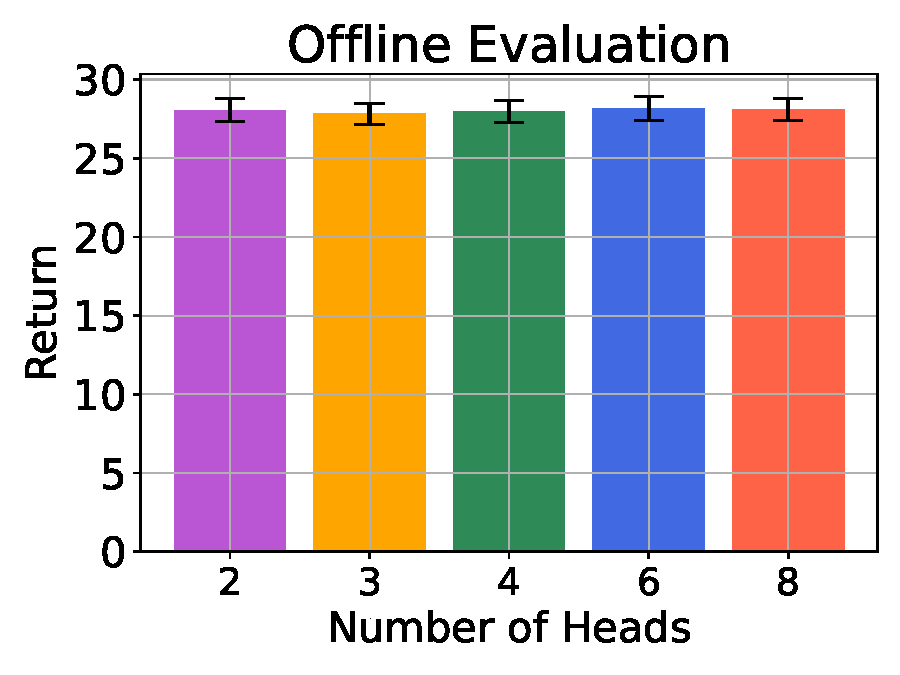
\includegraphics[width=0.25\columnwidth]{figures/plot_offline_different_head.pdf}  
% \!\!\!\!
% 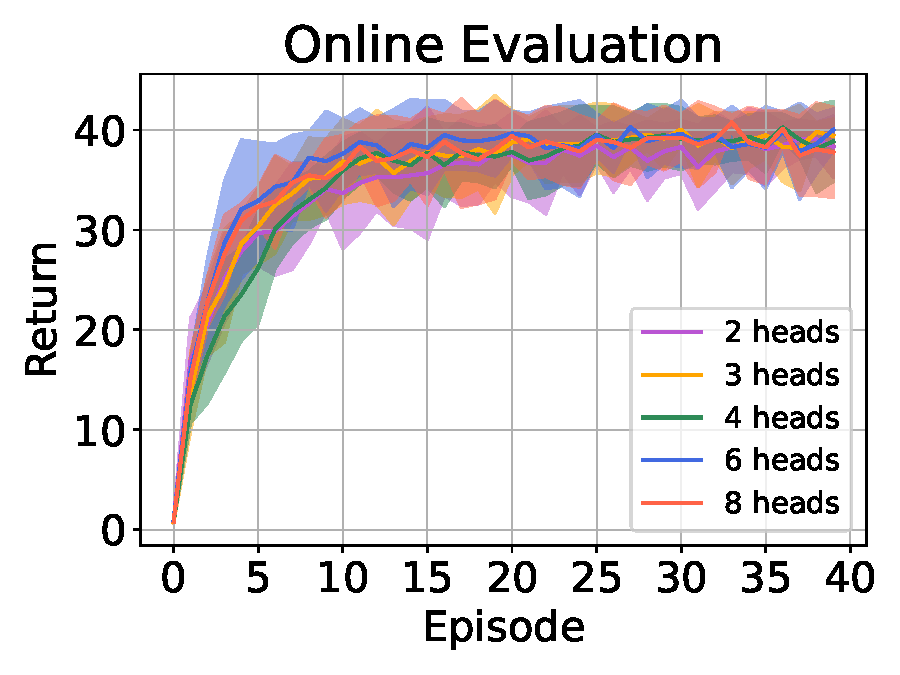
\includegraphics[width=0.25\columnwidth]{figures/plot_online_different_head.pdf}
% \!\!\!\!
% 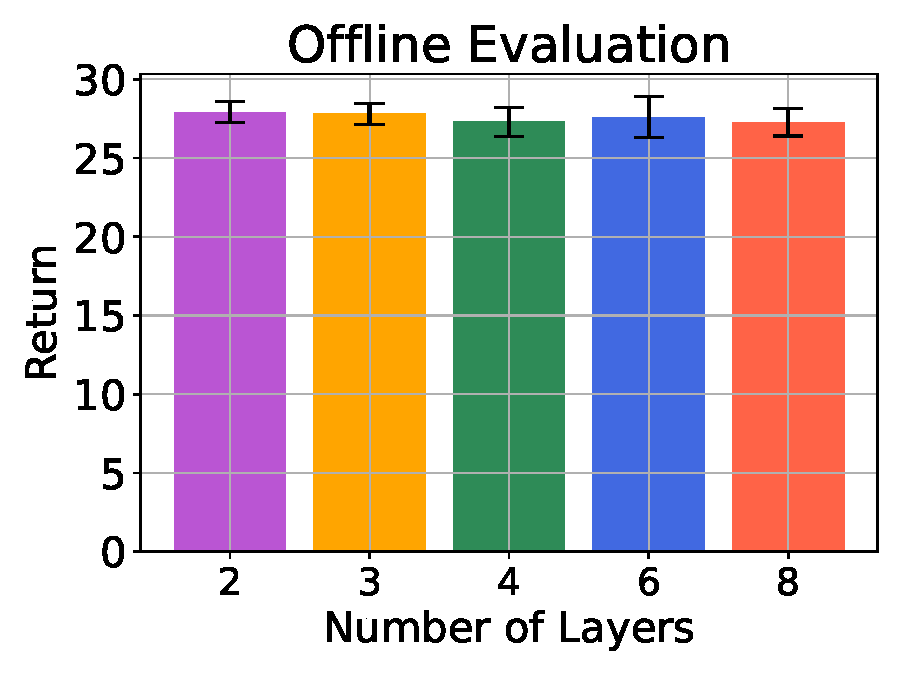
\includegraphics[width=0.25\columnwidth]{figures/plot_offline_different_layer.pdf} 
% \!\!\!\!
% 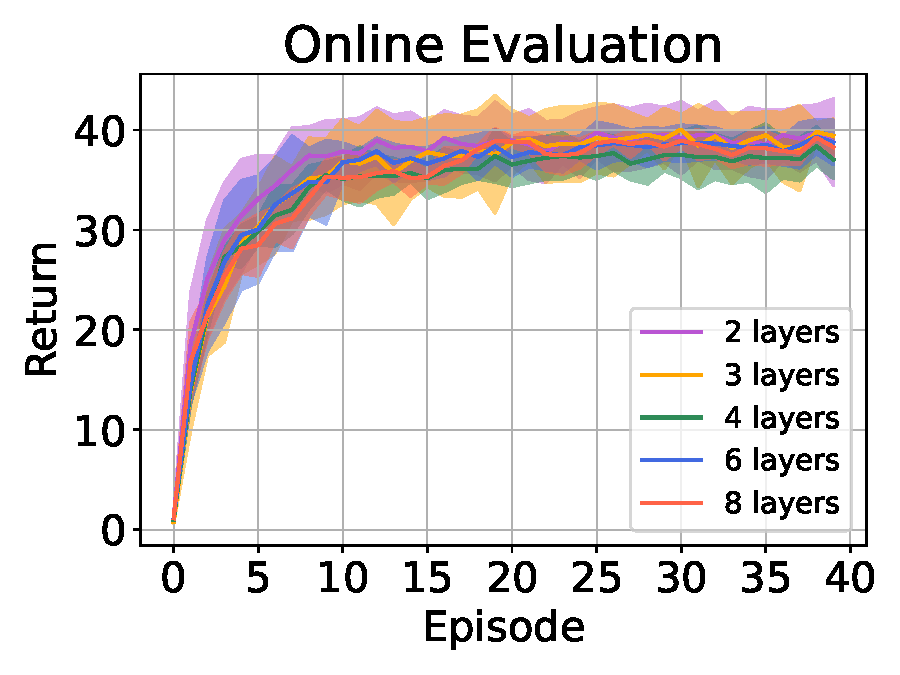
\includegraphics[width=0.25\columnwidth]{figures/plot_online_different_layer.pdf}  
% % \Description{DarkRoom}
% \caption{Offline and online evaluations of SAD with different transformer hyperparameters: the number of attention heads (left two), the number of attention layers (right two). Each hyperparameter contains four independent runs with mean and standard deviation.
% }
% \label{fig_diff_head_layer}
% \end{figure}


%%%%%%%%%%%%%%%%
\begin{figure}[ht]
\centering 
\setcounter{subfigure}{0}
\subfigure[]
{
	\begin{minipage}{0.25\linewidth}
	\centering 
	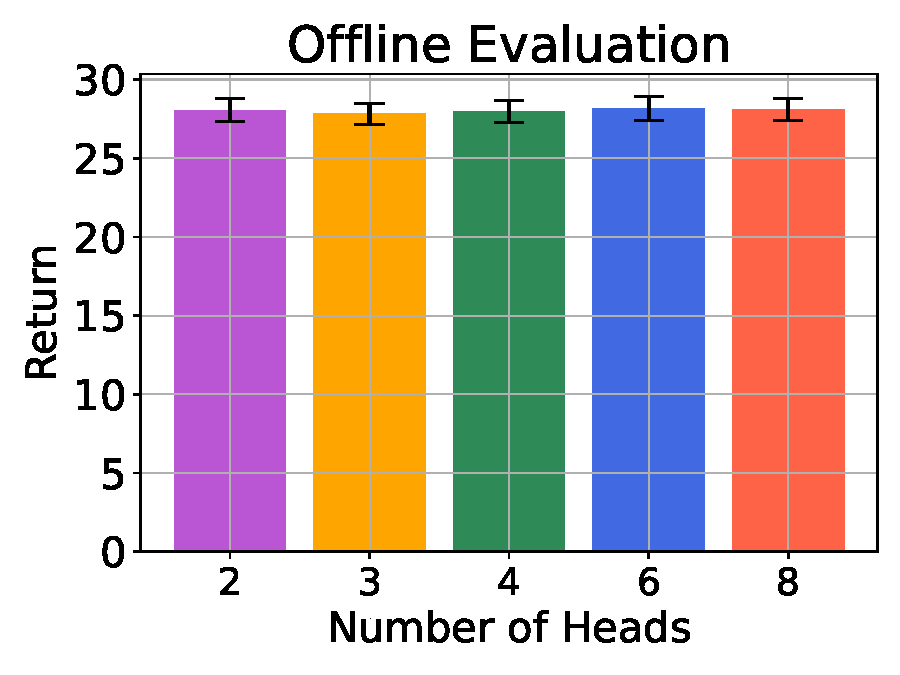
\includegraphics[width=\columnwidth]{figures/plot_offline_different_head.pdf}
	\end{minipage}
}
\!\!\!\!\!\!\!\!\!
\subfigure[]
{
	\begin{minipage}{0.25\linewidth}
	\centering 
	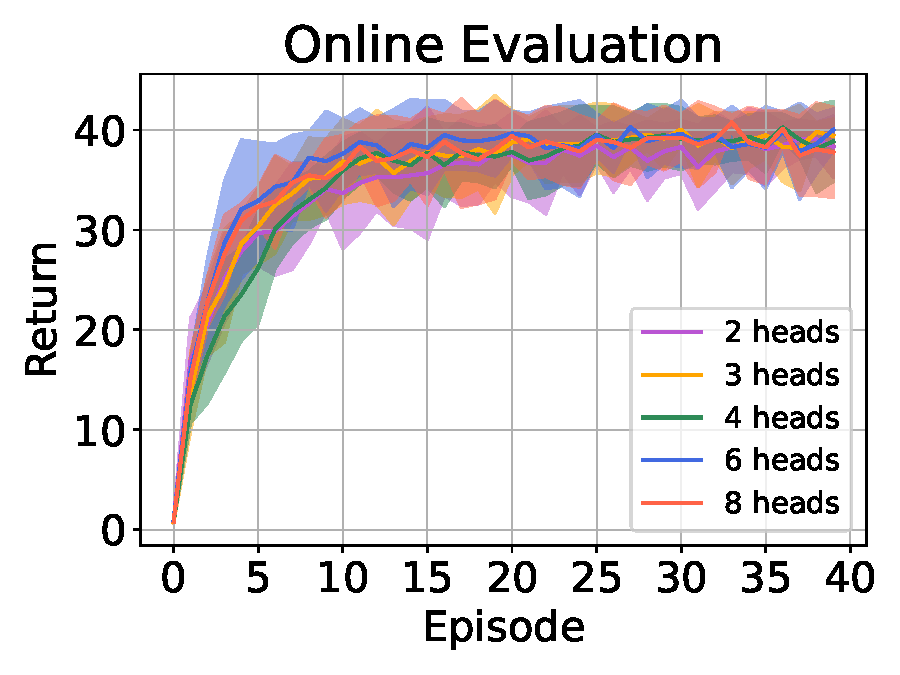
\includegraphics[width=\columnwidth]{figures/plot_online_different_head.pdf}
	\end{minipage}
}
\!\!\!\!\!\!\!\!\!
\subfigure[]
{
	\begin{minipage}{0.25\linewidth}
	\centering 
	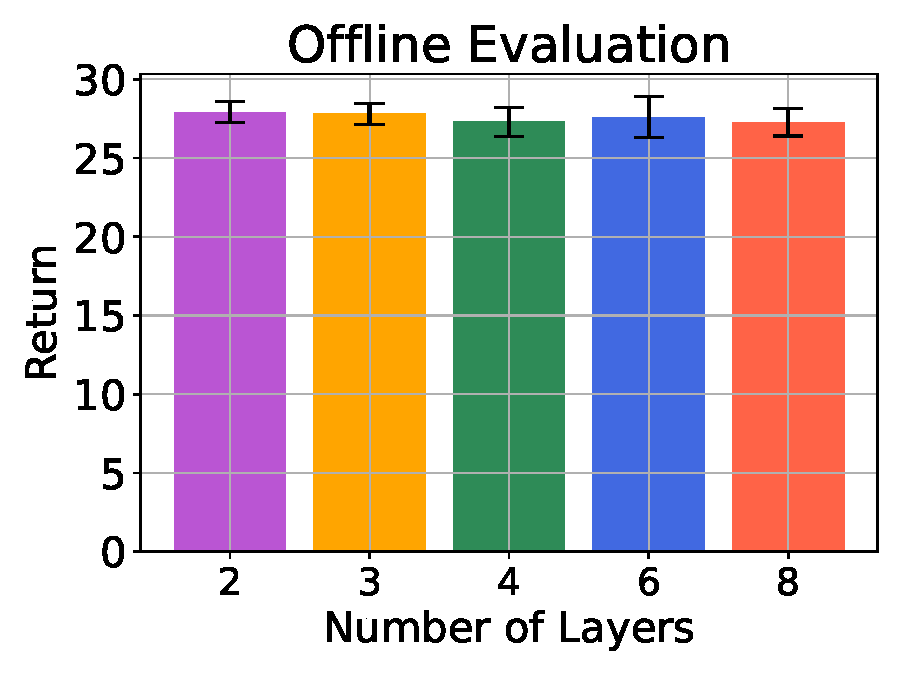
\includegraphics[width=\columnwidth]{figures/plot_offline_different_layer.pdf}
	\end{minipage}
}
\!\!\!\!\!\!\!\!\!
\subfigure[]
{
	\begin{minipage}{0.25\linewidth}
	\centering 
	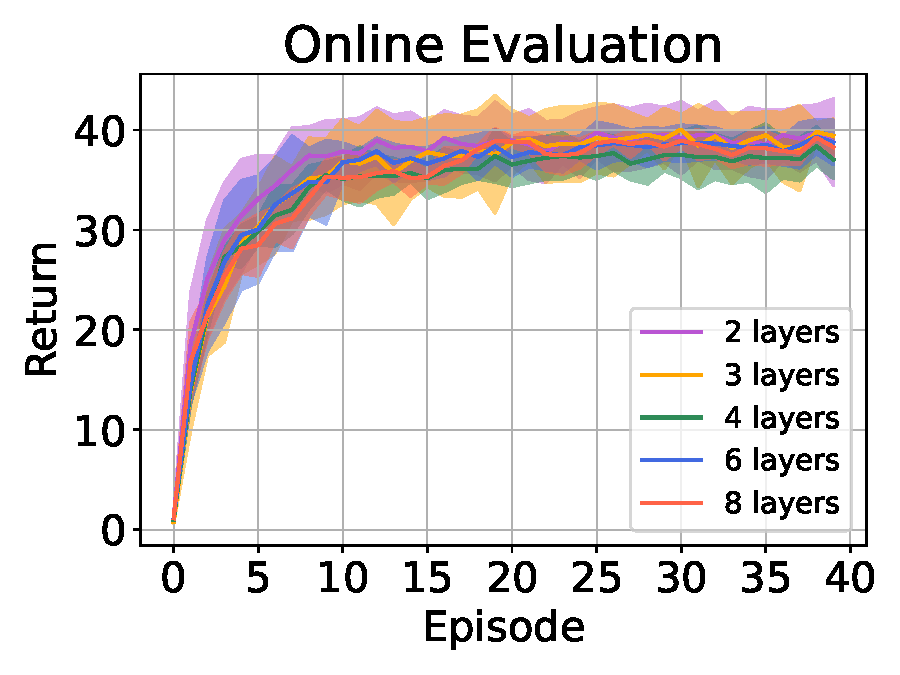
\includegraphics[width=\columnwidth]{figures/plot_online_different_layer.pdf}
	\end{minipage}
}
\caption{Offline and online evaluations of SAD with different transformer hyperparameters: the number of attention heads ((a) and (b)); the number of attention layers ((c) and (d)). Each hyperparameter contains four independent runs with mean and standard deviation.
}
\label{fig_diff_head_layer}
\end{figure}
%%%%%%%%%%%%%%%%



























%%%%%%%%%%%%%%%%%%%%%%%%%%%%%%%%%%%%%%%%%%%%%%%%%%%%%%%%%%%%%%%%%%%%%%%%
